\chapter{Experiment settings}
In this chapter, we evaluate the performance of our proposed metric and compare it with XQDA and NFST. We apply the proposed metric that is based on the KLFDA and gradient descent method to the GOG descriptor by a few steps. First, due to the high dimension of extracted GOG descriptors, KLFDA is applied to GOG descriptor to reduce the dimension to $C-1$, where $C$ is the number of person pairs in the training dataset. A transformation matrix $\bm{T}$ is generated in the dimension reduction. Second, with the dimension-reduced descriptors, a $(C-1) \times (C-1)$-dimensional SPD matrix $\bm{M}$ is trained based on the relative distance comparison, which restricts that the maximum intraclass distance is at least one unit smaller than the minimum interclass distance. The gradient descent method is used to optimize this problem by minimizing the target function \ref{TargetFunc2} in Chapter 4. At last, the matrix $\bm{T}$ is used to reduce the dimension of testing data to $(C-1)$-dimensional vectors. With the trained SPD matrix $\bm{M}$, we compute the similarity scores and CMCs of the testing data.
	
The XQDA and NFST are two metrics used to compare with our proposed metric in this thesis. A brief introduction of these two metrics is given in Chapter 2. These two metrics are chosen because they outperform most of the other previous metrics. The detailed comparison can be found in \cite{GOG} and \cite{NFST}. Also, in this thesis, XQDA and NFST are tested with the GOG descriptor to reduce possible errors that may be caused by using different descriptors.

\section{Datasets and evaluation settings}

\noindent \textbf{VIPeR} dataset is the most widely used dataset in person re-identification. In this dataset, there are 632 different individuals, and for each person, there are two outdoor images from different viewpoints. All the images are scaled into $48\times128$. In this experiment, we randomly select 316 individuals from cam A and cam B as the training set. The rest of the images in cam A are used as probe images, and those in cam B are used as gallery images. This process is repeated 10 times to reduce error.\\
%\textbf{ETHZ dataset} Three video sequences are contained in this dataset. In ETHZ there are respectively 83,35,28 persons in each sequences. All those images are outdoor and the camera is moving with the pedestrian. Images are in different sizes and may needed to resized. All those images of a certain person is shot with the same moving camera. In this paper, for each person two random images are selected as the training pair and another two random images are selected as the gallery and probe image.\\
\textbf{CUHK1} dataset contains 971 identities from two disjointed camera views. The cameras are static in each view, and images are listed in the same order. For each individual, there are two images in each view. All images are scaled into $60\times160$. In this paper, we randomly select 485 image pairs as training data, and the remaining pairs are used for test data. 
\begin{figure}[H]
\begin{raggedleft}
\includegraphics[width=1\linewidth]{/Users/JohnsonJohnson/Downloads/thesis_1/Figures/CUHKimagesdemo.jpg}
\vspace{-3em}
\caption{Pedestrians in prid\_450 dataset}
\end{raggedleft}
\end{figure}
\noindent\textbf{Prid\_2011} dataset consists of images extracted from multiple person trajectories recorded from two different, static surveillance cameras. Images from these cameras contain a viewpoint change and a stark difference in illumination, background and camera characteristics. Camera view A shows 385 persons, and camera view B shows 749 persons. The first 200 persons appear in both camera views. The remaining persons in each camera view complete the set of the corresponding view. In this paper, we randomly select 100 persons that appeared in both camera views as training pairs, and the remaining 100 persons of the 200 person pairs from camera A are used as the probe set while the 649 remaining persons from camera B are used for the gallery set.\\
%\begin{figure}[H]
%\begin{raggedleft}
%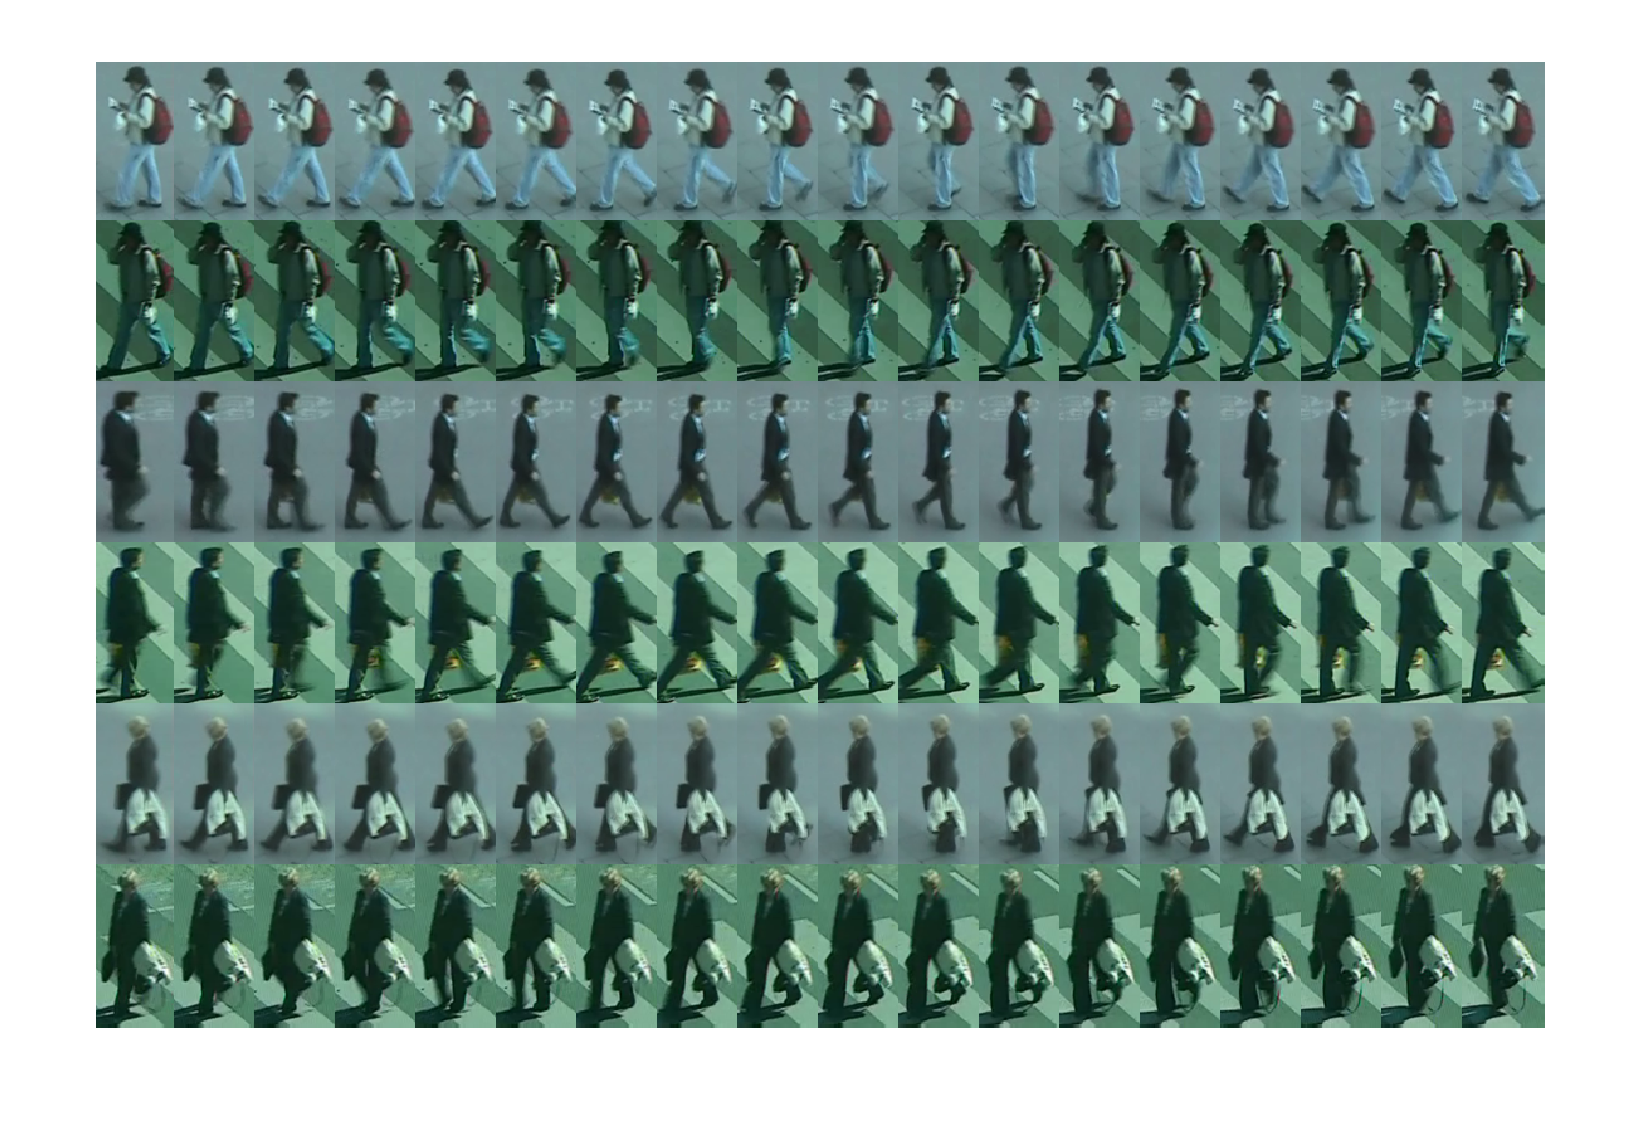
\includegraphics[width=1\linewidth]{/Users/JohnsonJohnson/Downloads/thesis_1/Figures/Multishots.eps}
%\vspace{-3em}
%\caption{Pedestrians in prid\_2011 dataset}
%\end{raggedleft}
%\end{figure}
%\label{Prid\_2011 pedestrians}
\textbf{Prid\_450s} dataset contains 450 image pairs recorded from two different, static surveillance cameras. Additionally, the dataset also provides an automatically generated, motion-based foreground/background segmentation as well as a manual segmentation of parts of a person. The images are stored in two folders that represent the two camera views. Besides the original images, the folders also contain binary masks obtained from motion segmentation, and manually segmented masks. In this test, we randomly select 225 persons from each of two camera views as the training set, and the remaining persons are left as the gallery and probe images. 
\begin{figure}[H]
\begin{raggedleft}
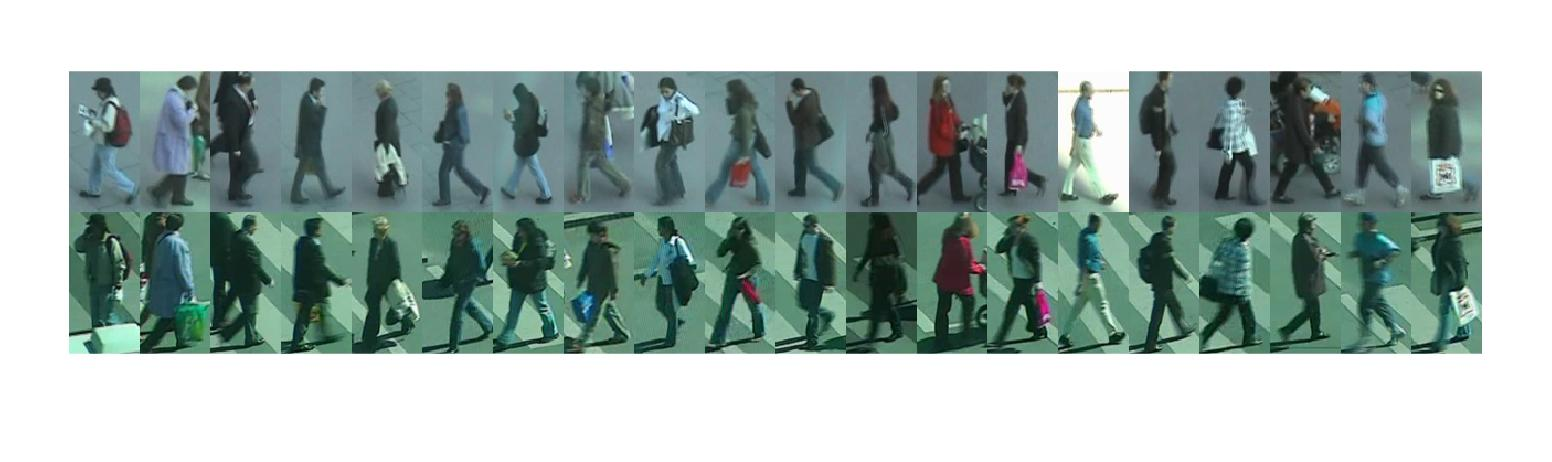
\includegraphics[width=1\linewidth]{/Users/JohnsonJohnson/Downloads/thesis_1/Figures/Prid450sImages.jpg}
\vspace{-3em}
\caption{Pedestrians in prid\_450s dataset}
\end{raggedleft}
\end{figure}
\noindent\textbf{GRID} has two camera views. The probe folder contains 250 probe images captured in one view (file names starts from 0001  to 0250). The gallery folder contains 250 true match images of the probes (file names starts from 0001  to 0250). Furthermore, in the gallery folder, there are a total of 775 additional images that do not belong to any of the probes (file name starts with 0000). These extra images should be treated as a fixed portion in the testing set during cross validation. In this paper, we randomly select 125 persons from those 250 persons who appeared in both camera views as training pairs, and the remaining persons in the probe folder are used as probe images while  the remaining 125 persons and those 775 additional persons from the gallery folder are used as gallery images. A brief summarization of test settings of all those datasets mentioned is listed in Table \ref{Settings}.

\begin{figure}[H]
\begin{raggedleft}
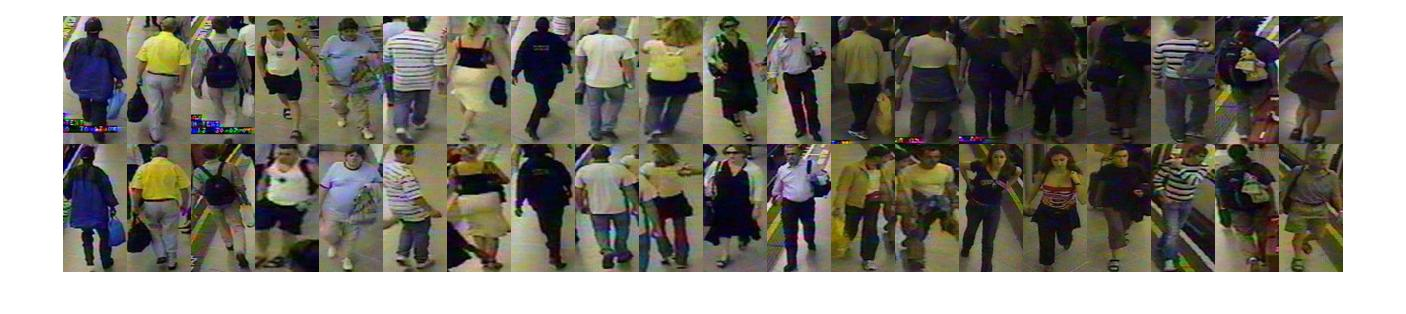
\includegraphics[width=1\linewidth]{/Users/JohnsonJohnson/Downloads/thesis_1/Figures/GRIDimagesdemo.jpg}
\vspace{-3em}
\caption{Pedestrians in GRID dataset}
\end{raggedleft}
\end{figure}
%-------------------------------------------------
\begin{table}[H]
\centering
\caption{Testing setting for different datasets}
\label{Settings}
%\centering
\begin{tabular}{|l|c|c|c|c|c|}
\hline
Dataset&training&probe&gallery&cam\_a&cam\_b\\
\hline
VIPeR&316&316&316&632&632\\
\hline
CUHK1&485&486&486&971&971\\
\hline
Prid\_2011&100&100&649&385&749\\
\hline
Prid\_450s&225&225&225&450&450\\
\hline
GRID&125&125&900&250&1025\\
\hline
\end{tabular}\\ 
\end{table}
%-----------------------------------------------------------------------------------------------------------------------------------------------------------------------------------------------------------------------------------------------------
\section{The influence of mean removal and $L_2$ normalization}
In \cite{GOG}, mean removal and $L_2$  normalization is found to improve performance by $5.1\%$. The reason for this is that mean removal and normalization can reduce the impact of extremas of descriptors. When testing proposed metric learning, we find that mean removal can slightly improve performance. A comparison between performances of original descriptors and preprocessed descriptors is shown in Tables \ref{table:compMN1}, \ref{table:compMN2}, \ref{compMN3}, \ref{compMN4} and \ref{compMN5}, and all those datasets are tested by proposed metric. The original GOG means no mean removal and normalization. It shows that the mean removal and normalization has a slight improvement of around 0.5\% on the performance on all five datasets. Since preprocessing is required to test XQDA, the mean removal and normalization are applied on descriptors in this experiment. 

\begin{table}[H]
\centering
\caption{The influence of data preprocessing on VIPeR}
\label{table:compMN1}
\begin{tabular}{|l|c|c|c|c|c|}
\hline
 & \multicolumn{5}{|c|}{Rank(\%)} \\
 \hline
Terms  &1 &5 & 10 &15& 20\\
\hline
Original GOG &43.01&74.91& 84.87& 89.81& 93.32 \\
\hline
Preprocessed GOG$_\text{rgb}$ &43.77&74.84&85.25& 90.32&93.89\\
 \hline
Original GOG$_\text{fusion}$ &48.77&77.47&87.41&91.52&94.27\\
\hline
Preprocessed GOG$_\text{fusion}$ &48.32&76.90&87.78&91.93& 94.49\\
 \hline

\end{tabular}
\end{table}


%---------------------------------------------
\begin{table}[H]
\centering
\caption{The influence of data preprocessing on CUHK1}
\label{table:compMN2}
\begin{tabular}{|l|c|c|c|c|c|}
\hline
 & \multicolumn{5}{|c|}{Rank(\%)} \\
 \hline
Terms  &1 &5 & 10 &15& 20\\
\hline
Original GOG$_\text{rgb}$&56.11&83.77&90.10& 92.65&94.28 \\
\hline
Preprocessed GOG$_\text{rgb}$ &55.91&84.24&90.41& 93.15&94.67\\
 \hline
Original GOG$_\text{fusion}$ &57.10&84.65& 90.35& 92.88&94.65\\
\hline
Preprocessed GOG$_\text{fusion}$ &56.67&84.49& 90.51& 93.31&94.84\\
 \hline
 
\end{tabular}
\end{table}

%---------------------------------------------
\begin{table}[H]
\centering
\caption{The influence of data preprocessing on prid\_2011}
\label{compMN3}
\begin{tabular}{|l|c|c|c|c|c|}
\hline
 & \multicolumn{5}{|c|}{Rank(\%)} \\
 \hline
Terms  &1 &5 & 10 &15& 20\\
\hline
Original GOG$_\text{rgb}$&24.80& 52.10& 63.20& 69.90& 72.90\\
\hline
Preprocessed GOG$_\text{rgb}$ &23.80& 52.20& 63.50& 70.20& 73.50\\
\hline
Original GOG$_\text{fusion}$ &32.20& 56.60& 67.00& 73.10& 77.70\\
\hline
Preprocessed GOG$_\text{fusion}$ &32.30& 57.40& 66.30& 73.40& 78.00\\
 \hline
 
\end{tabular}
\end{table}

%---------------------------------------------
\begin{table}[H]
\centering
\caption{The influence of data preprocessing on prid\_450s}
\label{compMN4}
\begin{tabular}{|l|c|c|c|c|c|}
\hline
 & \multicolumn{5}{|c|}{Rank(\%)} \\
 \hline
Terms  &1 &5 & 10 &15& 20\\
\hline
Original GOG$_\text{rgb}$&60.93& 84.31& 91.29& 94.00& 96.18\\
\hline
Preprocessed GOG$_\text{rgb}$ &60.71& 84.53& 91.29& 94.13& 96.27\\
\hline
Original GOG$_\text{fusion}$ &63.07& 86.67& 92.53& 95.20& 96.98\\
\hline
Preprocessed GOG$_\text{fusion}$ &62.80& 86.58& 92.36& 95.29& 96.89\\
 \hline
 
\end{tabular}
\end{table}

%---------------------------------------------
\begin{table}[H]
\centering
\caption{The influence of data preprocessing on GRID}
\label{compMN5}
\begin{tabular}{|l|c|c|c|c|c|}
\hline
 & \multicolumn{5}{|c|}{Rank(\%)} \\
 \hline
Terms  &1 &5 & 10 &15& 20\\
\hline
Original GOG$_\text{rgb}$&22.96& 41.92& 51.68& 58.72& 64.64\\
\hline
Preprocessed GOG$_\text{rgb}$ &22.64& 43.68& 52.00& 59.04& 65.04\\
\hline
Original GOG$_\text{fusion}$ &24.32& 44.56& 54.80& 62.40& 66.64\\
\hline
Preprocessed GOG$_\text{fusion}$ &23.92& 44.64& 54.88& 62.32& 66.40\\
 \hline
 
\end{tabular}
\end{table}


%--------------------------------------------------
\section{Parameters setting}
In this experiment, there are a few parameters for the iteration computing, including slack variable $\rho$, maximal iteration $T$, gradient step $\lambda$, the interclass and intraclass limitation factor $\alpha$ and the updating ratio $\beta$. First, the slack variable $\rho$ is initialized as 1 to ensure the minimum interclass distance is 1 larger than intraclass distance at least. The step size of gradient updating $\lambda$ is initialized as 0.01. When target value $f$ increases,  $\lambda$ is scaled by a factor of 0.5, and  $\lambda$ is scaled by 1.01 when target value $f$ decreases. To judge if target value converges, the threshold $\beta$ is defined as the ratio target value change versus previous target value, that is, $\beta = \frac{(f_{t+1}-f_t)}{f_t}$. According to many experiment trials, when it satisfies $\beta = 10^{-5}$, the target value converges and the iteration is stopped. The maximal iteration times $t$ is set to 100 since the target value $f$ will converge in around 15 iterations.  The last parameter for the iteration is $\alpha$. To know the best value for $\alpha$, we tried 11 different values ranges from 0 to 1 with a step of 0.1. We found that the rank 1 and rank 5 scores reach maxima at interval $[0.7,0.8]$, as shown in \ref{Rank1curve} and \ref{Rank5curve}. Then another ten trials were performed with alpha ranging from $[0.7,0.8]$ with a step of 0.01. The best $\alpha$ value should have largest top-ranking scores possible and at last we found that the optimal value for $\alpha$ is 0.76. A form of all parameters is shown in Table \ref{ParametersSetting}.
%-------------------------------------------------
\begin{figure}[H]
\begin{raggedleft}
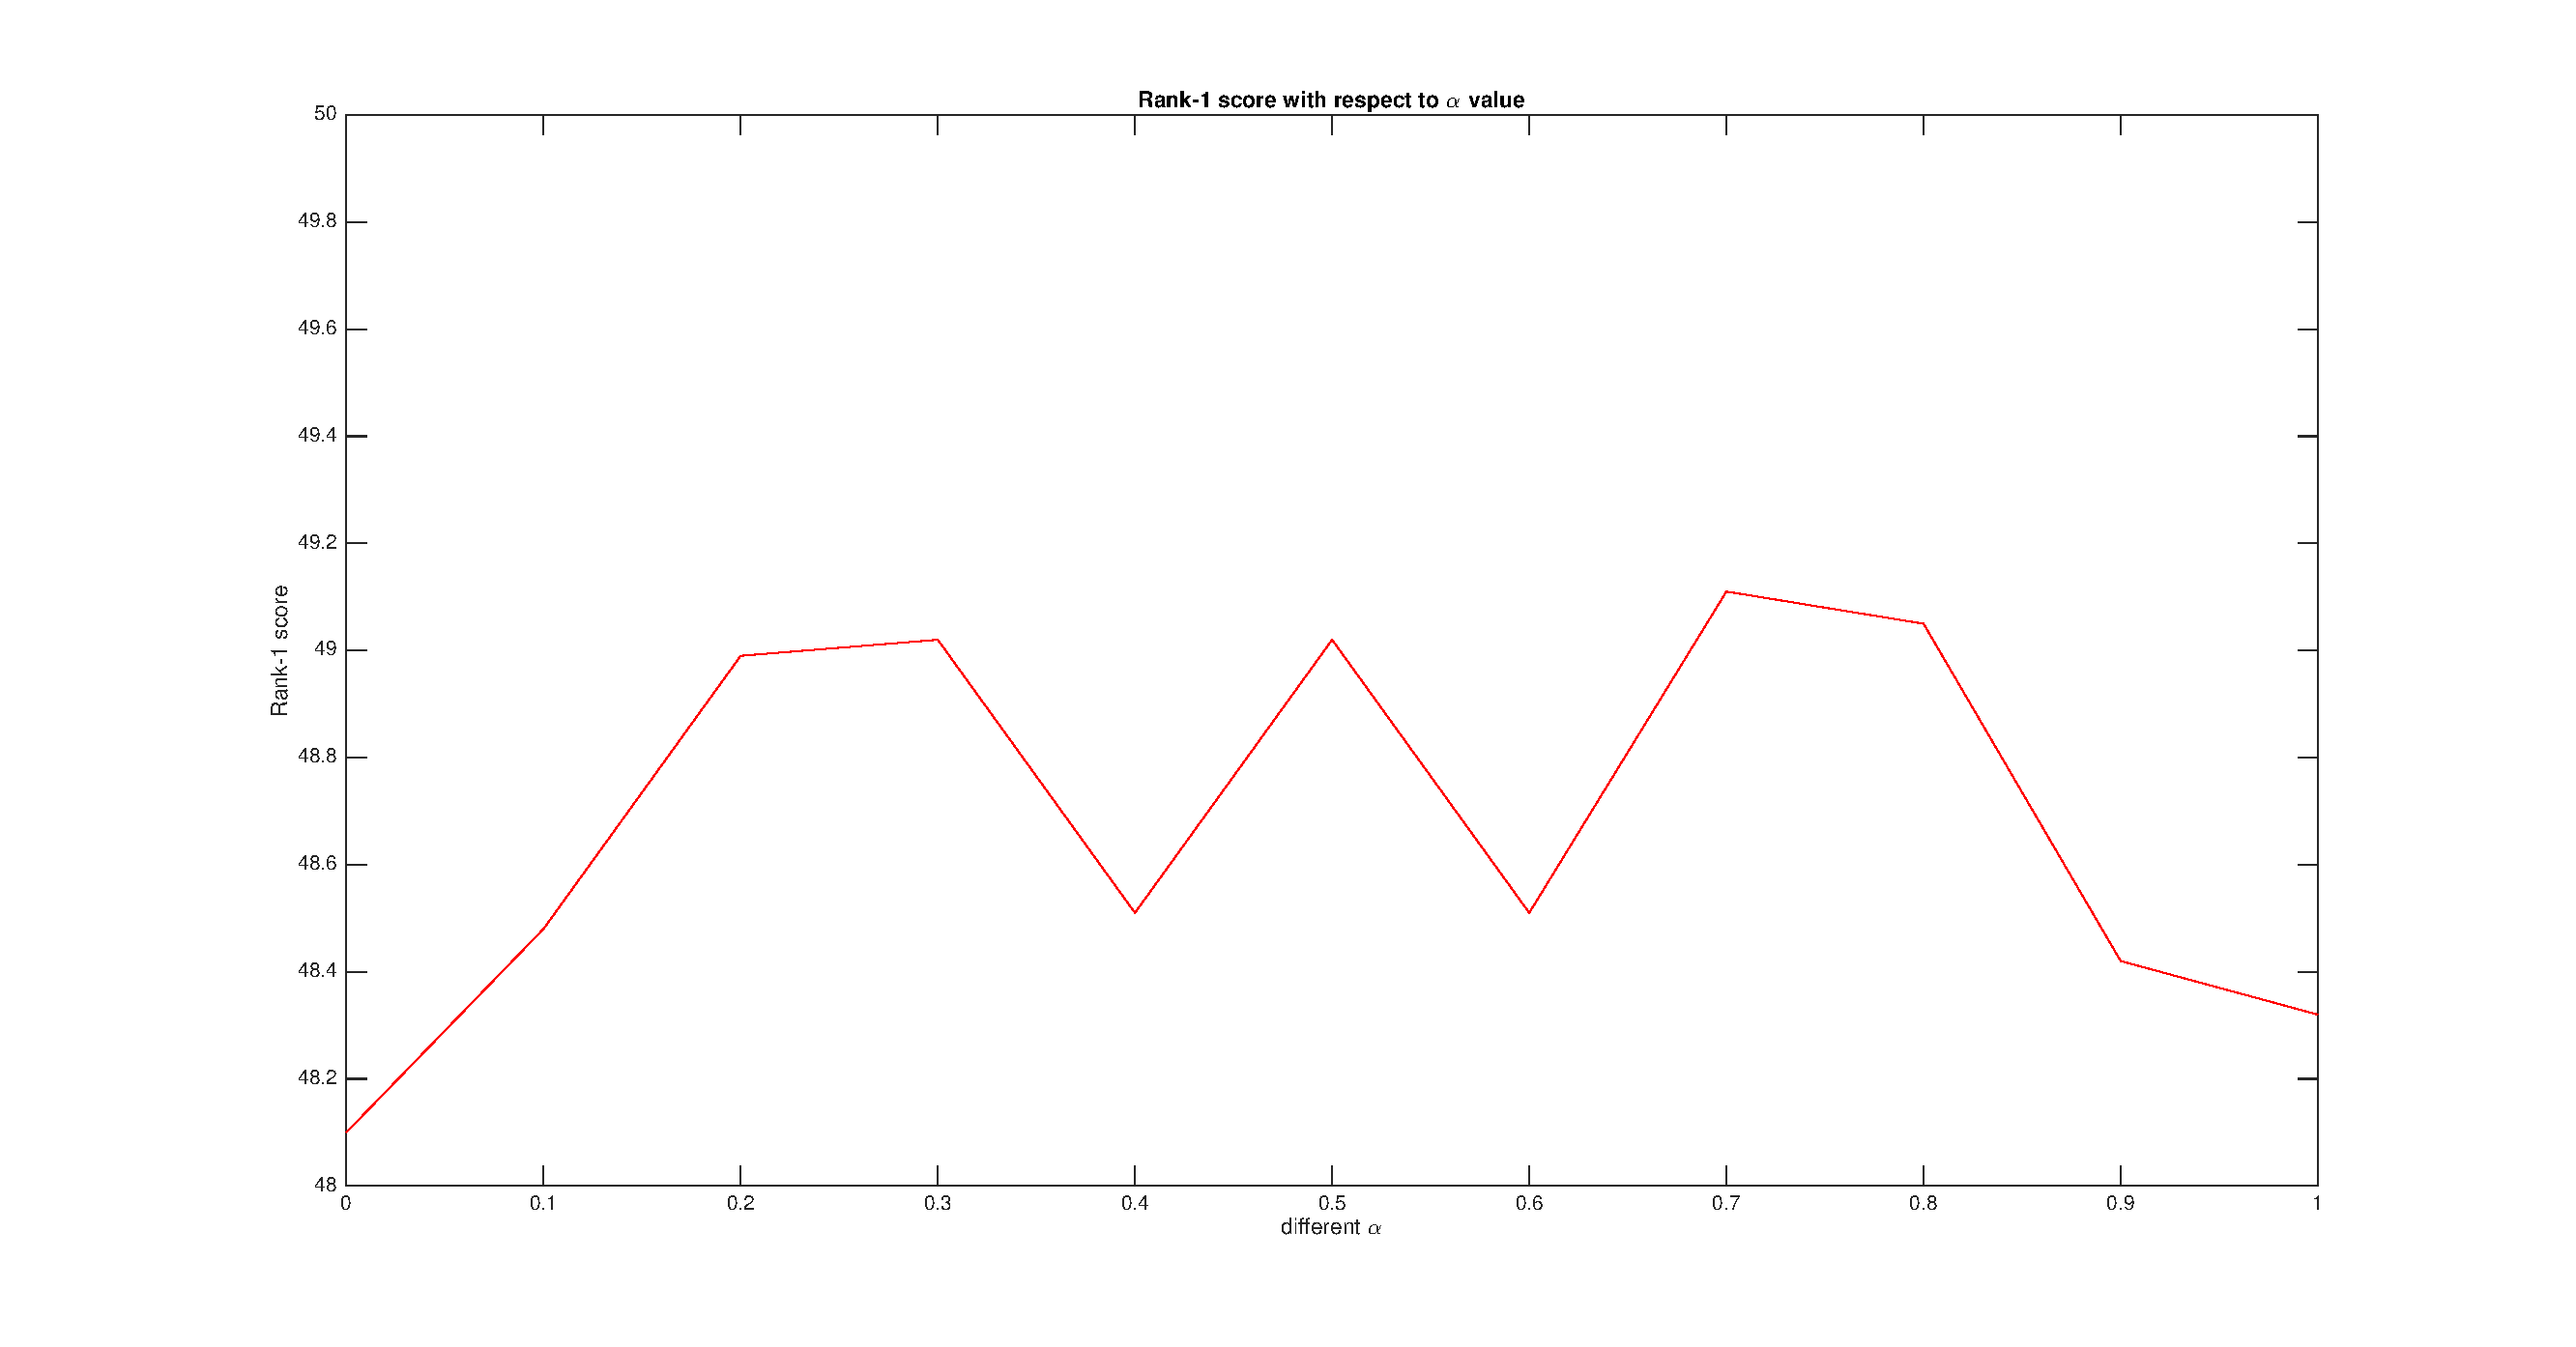
\includegraphics[width=1\linewidth]{/Users/JohnsonJohnson/Downloads/thesis_1/Figures/Rank1scoresAlpha.eps}
\vspace{-3em}
\caption{Rank 1 scores with respect to $\alpha$ on VIPeR}
\label{Rank1curve}
\end{raggedleft}
\end{figure}
%-------------------------------------------------
\begin{figure}[H]
\begin{raggedleft}
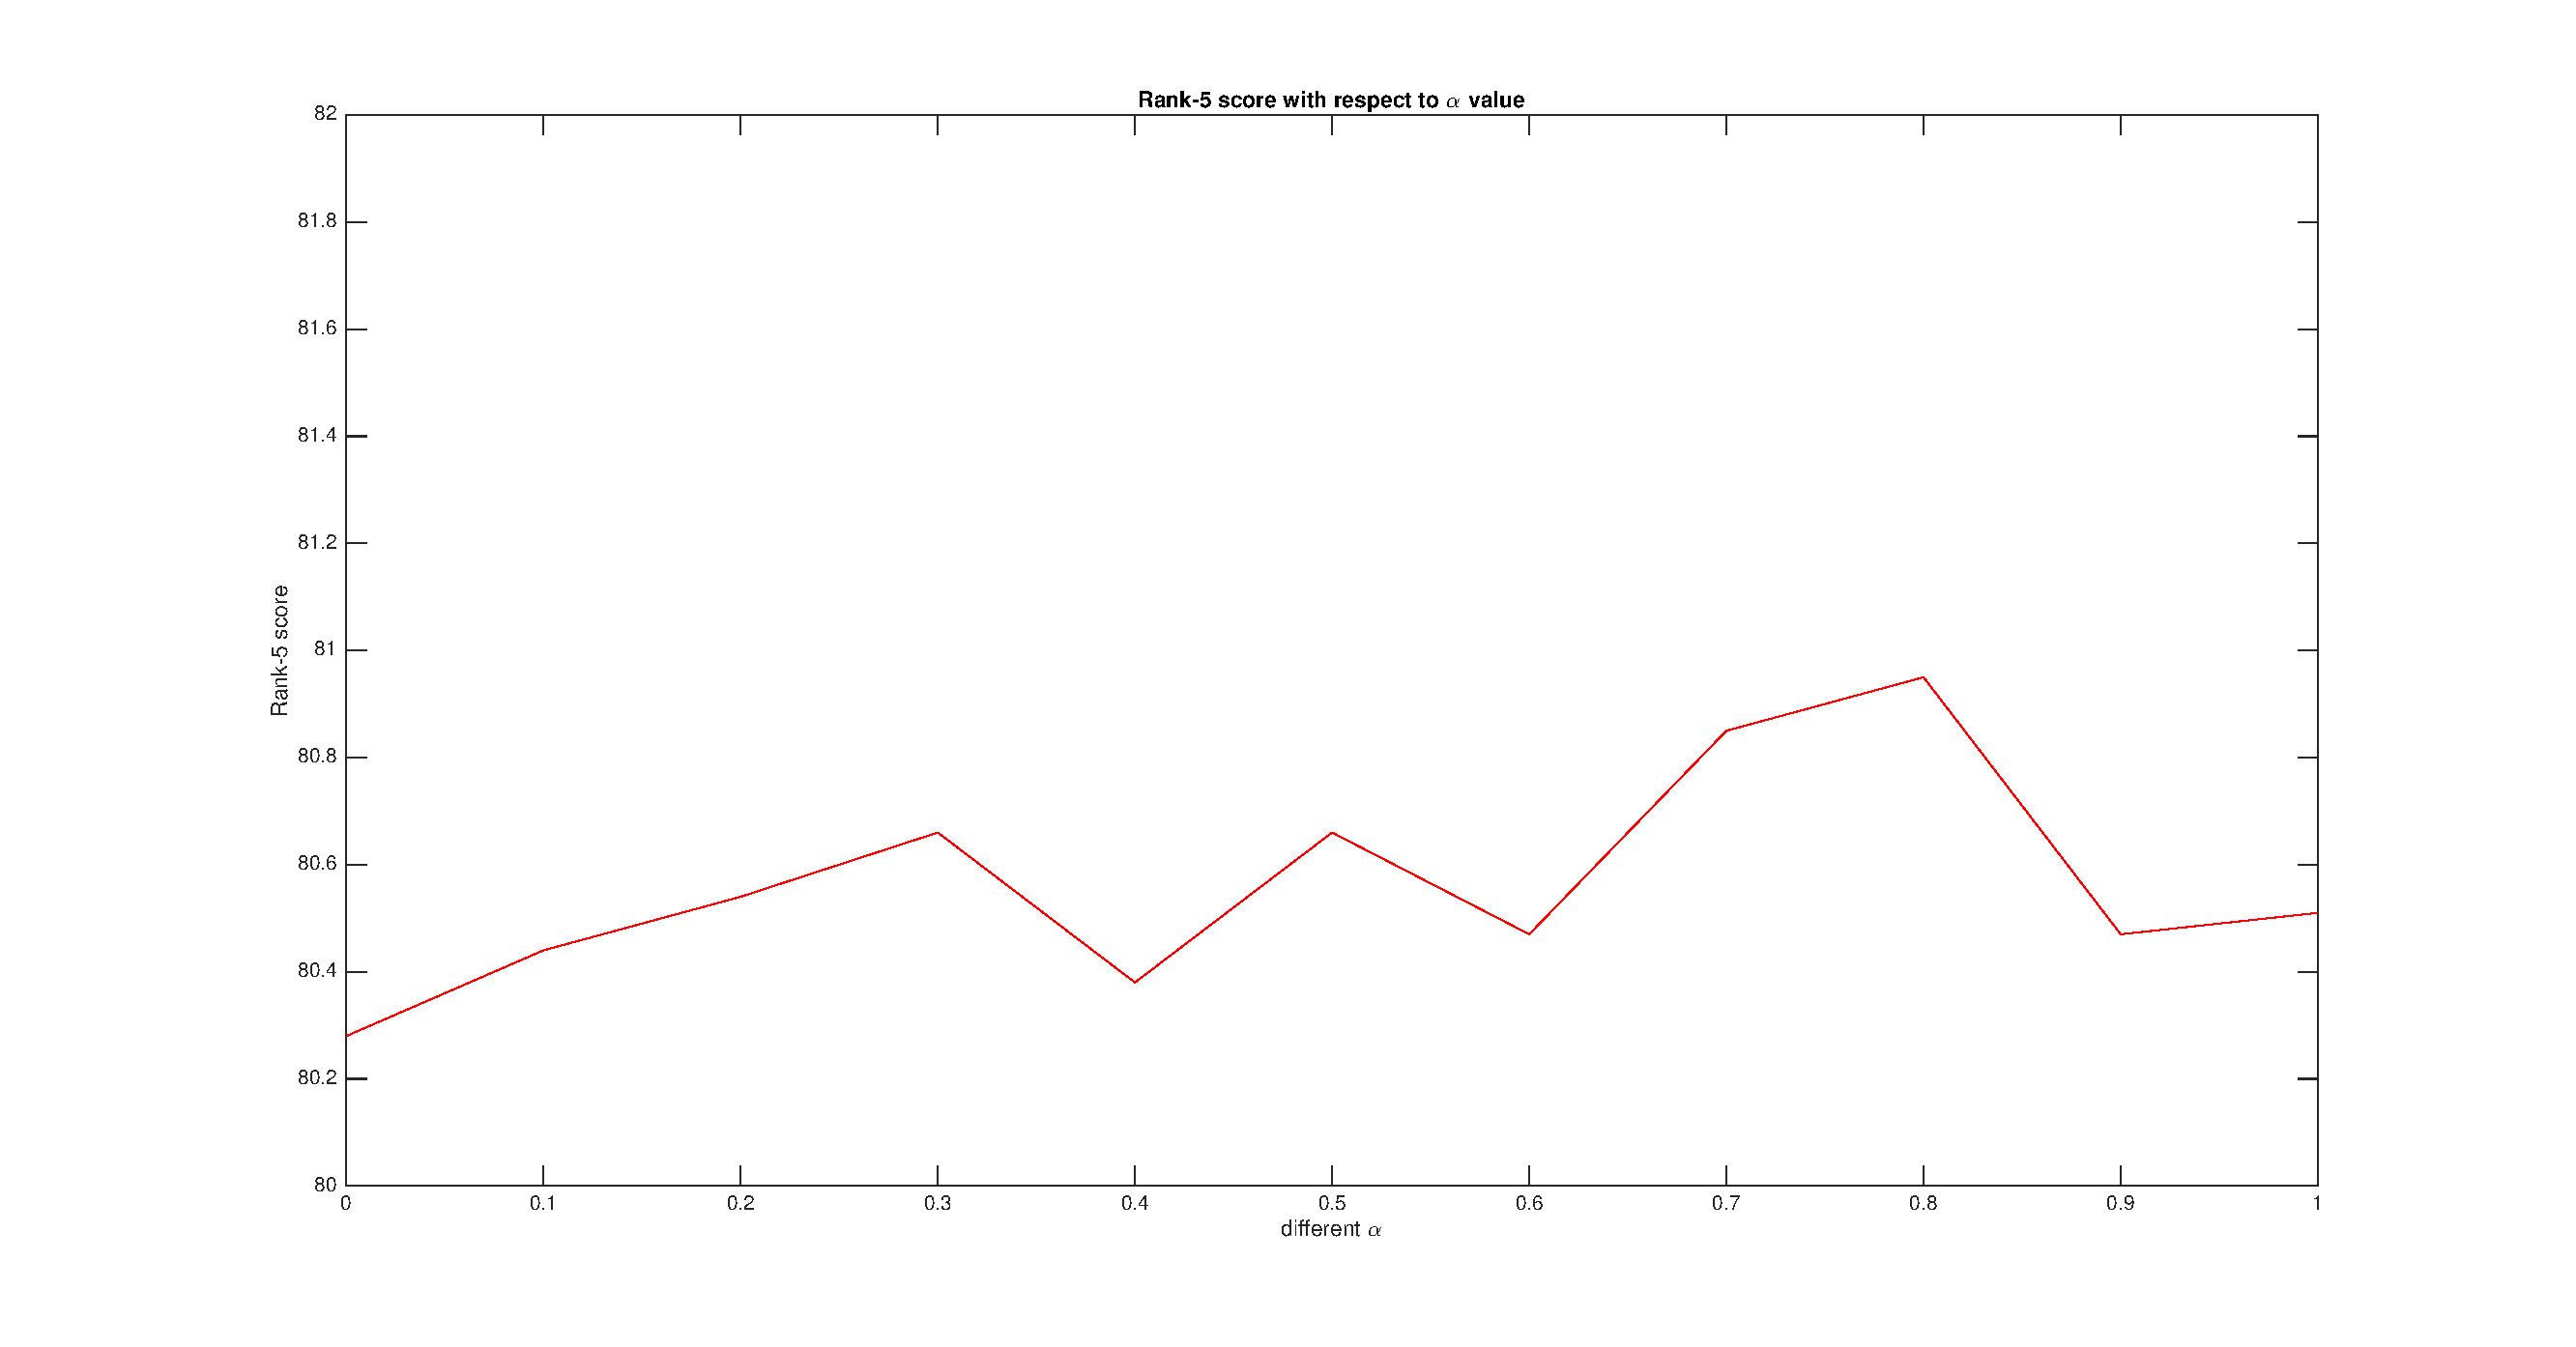
\includegraphics[width=1\linewidth]{/Users/JohnsonJohnson/Downloads/thesis_1/Figures/Rank5scoresAlpha.eps}
\vspace{-3em}
\caption{Rank 5 scores with respect to $\alpha$ on VIPeR}
\label{Rank5curve}
\end{raggedleft}
\end{figure}
%-------------------------------------------------

\begin{table}[H]
\centering
\caption{Parameters setting}
\label{ParametersSetting}
\begin{tabular}{|l|c|c|c|c|c|}
\hline
Paramters &$\alpha$&$\beta$&$\lambda$&$t$& $\rho$\\
\hline
Values &0.76&$10^{-5}$&0.01&100&1\\
\hline
\end{tabular}
\end{table}


\textbf{Performance measuring} The cumulative matching curve is used to measure the descriptor performance. The score means the probability that the right match is within the top $n$ samples. A better CMC is expected to have a high rank-1 value and reaches 1 as fast as possible.
%\section{XQDA and NFST}


\section{Results and experiment analysis}
In this paper, we compare proposed metric with other state-of-the-art metrics including NFST \cite{NFST} and XQDA \cite{LOMO}. NFST is a metric which enables us to learn a null space for descriptors so that the the same class descriptors will be projected to a single point to minimize within-class scatter matrix while different classes are projected to different points. This metric is a good solution to small sample problems in person re-identification. XQDA is quite similar to many other metrics, which learns a projection matrix $W$, and then a Mahalanobis SPD matrix $\bm{M}$ is learned in the subspace. These two metrics are proven to have state-of-the-art performance with many other methods. The GOG$_\text{rgb}$ in all forms stands for the hierarchical Gaussian descriptor in RGB color space, while GOG$_\text{fusion}$ stands for the descriptor concatenated by four different color spaces \{RGB, Lab, HSV, nRnG\}.\\
\indent\textbf{VIPeR} A comparison form is given in Table 3. Some of recent results are also included in this form. We can find that the rank scores are better than those of NFST and XQDA in terms of both GOG$_\text{rgb}$ and GOG$_\text{fusion}$. More specifically, the rank 1, rank 5, rank 10, rank 15 and rank 20 scores of proposed metric learning are 0.76\%, 0.92\%, 1.39\%, 1.08\%, 1.52\% higher than those of GOG$_\text{rgb}$ + XQDA. The rank 1, rank 5, rank 10, rank 15 and rank 20 GOG$_\text{fusion}$ scores of proposed metric learning are 0.35\%, -0.54\%, 0.98\%, 0.66\%, 0.79\% higher than GOG$_\text{fusion}$ + XQDA respectively. Also, we can see that proposed metric learning has a better performance than NFST. \newline 
%-----------------------------------------------------------------------VIPeR
\begin{table}[H]
\caption{Performance of different metrics on VIPeR}
\centering
 \begin{tabular}{|l|c|c|c|c|c|c|}
\hline
& \multicolumn{5}{|c|}{Rank(\%)} \\
\hline
Methods& 1 & 5 &10& 15&20\\
\hline
GOG$_\text{rgb}$+NFST& 43.23&73.16 &83.64 & 89.59&92.88\\  
\hline
GOG$_\text{rgb}$+XQDA& 43.01&73.92&83.86& 89.24& 92.37\\
\hline
%GOG$_\text{rgb}$+KLFDA&43.45 &74.68 &85.13 &90.54&93.70\\ 
%\hline
GOG$_\text{rgb}$+Proposed&43.77 &74.84&85.25&90.32&93.89\\   %43.48%, 74.59%, 85.35%, 90.47%, 93.67%
\hline
GOG$_\text{fusion}$+NFST&47.15& 76.39&87.31&91.74&94.49\\
\hline
GOG$_\text{fusion}$+XQDA& 47.97& 77.44& 86.80& 91.27&93.70\\  
\hline
%GOG$_\text{fusion}$+KLFDA & 47.97&77.06& 87.56&91.80&94.18\\
%\hline
GOG$_\text{fusion}$+Proposed&48.32&76.90&87.78&91.93&94.49\\ %48.16%, 76.65%, 87.66%, 91.90%, 94.37% 

\hline

%--------------------------------------------------------------
\end{tabular}
\end{table}
\textbf{CUHK1} We can find that the rank 1, rank 5, rank 10, rank 15 and rank 20 scores of GOG$_\text{rgb}$ combined with proposed metric are 5.4\%, 4.18\%, 3.31\%, 2.16\% and 1.46\% higher than XQDA, and 0.31\%, 1.22\%, 1.34\%, 1.17\% and 1.11\% higher than NFST.  Also, the  rank 1, rank 5, rank 10, rank 15 and rank 20 scores of GOG$_\text{fusion}$ combined with the proposed metric are 4.57\%, 2.64\%, 0.70\%, 1.33\% and 0.83\% higher than GOG$_\text{fusion}$ combined with XQDA, and 0.41\%, 0.83\%, 0.88\%, 1.09\% and 1.14\% than GOG$_\text{fusion}$ combined with NFST.  

\begin{figure}[H]
\begin{raggedleft}
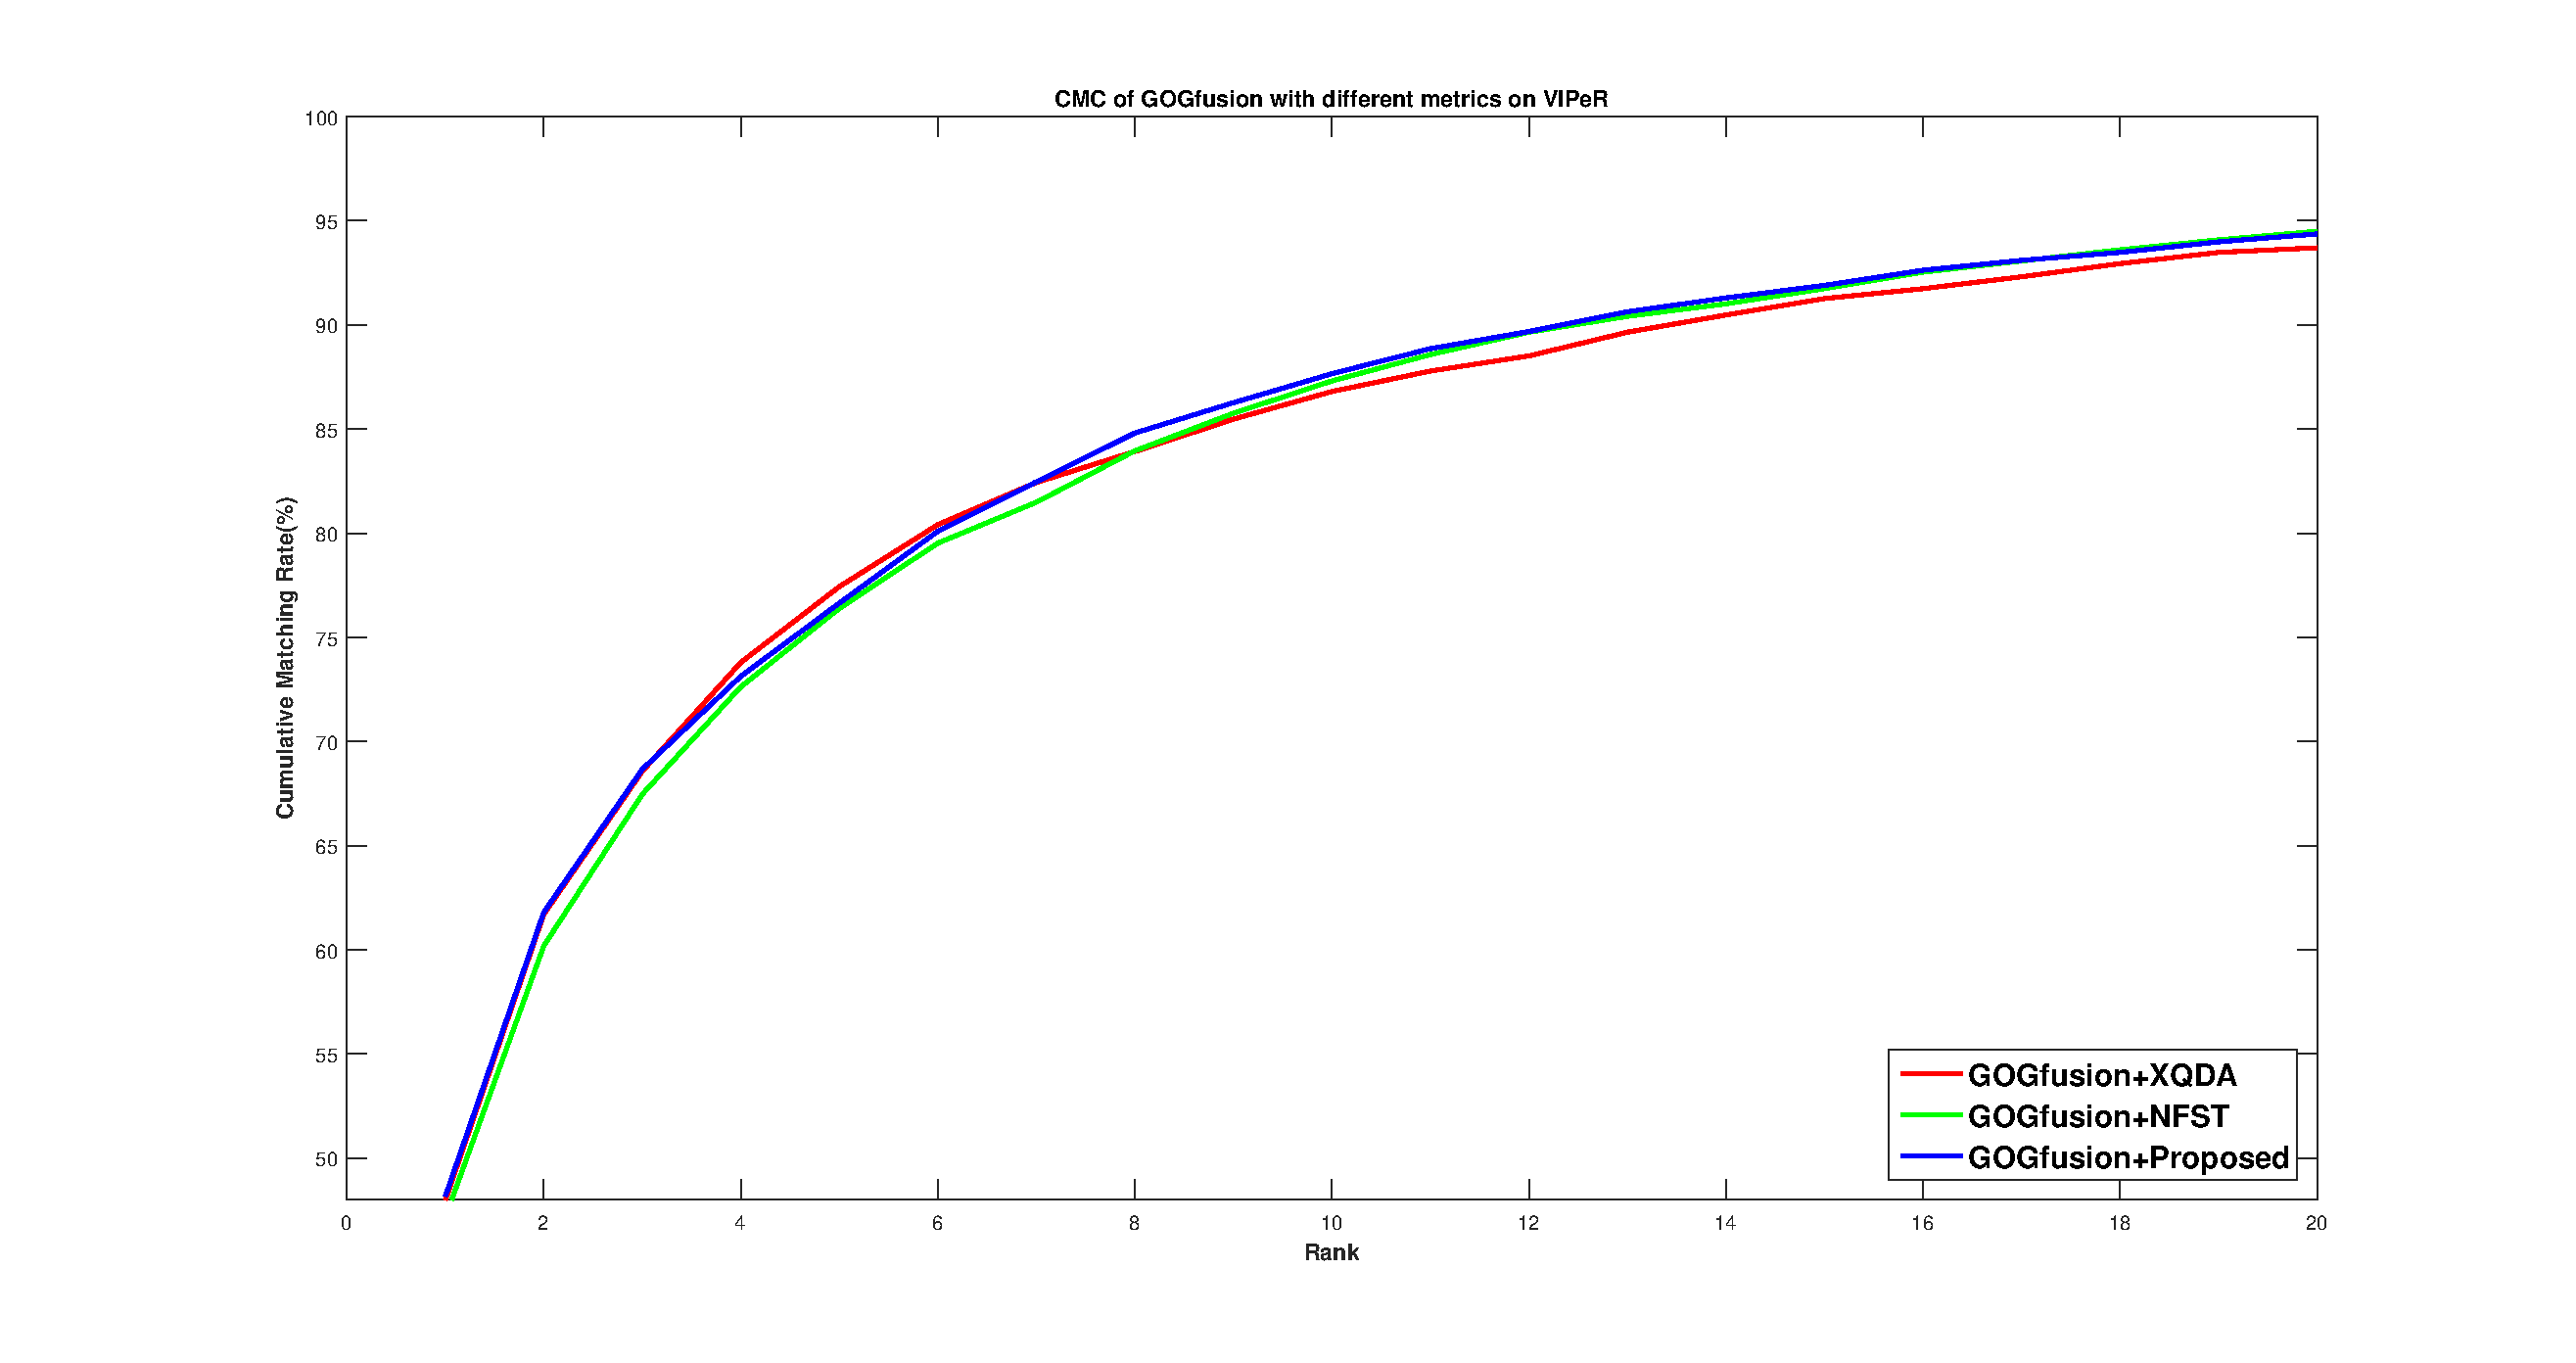
\includegraphics[width=1\linewidth]{/Users/JohnsonJohnson/Downloads/thesis_1/Figures/VIPeR.eps}
\vspace{-3em}
\caption{CMCs on VIPeR comparing different metric learning}
\end{raggedleft}
\end{figure}
%-------------------------------

%-----------------------------------------------------------------------CUHK1
\begin{table}[H]
\caption{Performance of different metrics on CUHK1}
\centering
\begin{tabular}{|l|c|c|c|c|c|c|}
\hline
& \multicolumn{5}{|c|}{Rank(\%)} \\
\hline
Methods& 1 & 5 &10&15& 20\\
\hline
GOG$_\text{rgb}$+NFST&55.60 &83.02 &89.07 &91.98&93.56 \\ 
\hline
GOG$_\text{rgb}$+XQDA&50.51 &80.06 &87.10 &90.99&93.21 \\ 
\hline
%GOG$_\text{rgb}$+KLFDA&55.66&84.32&90.66&93.07& 94.63\\
%\hline
GOG$_\text{rgb}$+Proposed&55.91&84.24&90.41& 93.15&94.67\\  %55.86%, 84.28%, 90.45%, 93.09%, 94.65% 
\hline
GOG$_\text{fusion}$+NFST&56.26 &83.66 &89.63 &92.22&93.70 \\ 
\hline
GOG$_\text{fusion}$+XQDA&52.10 &81.85&88.81 &91.98&94.01\\ 
\hline
%GOG$_\text{fusion}$+KLFDA & 56.60&84.67&90.41&93.13&94.81\\
%\hline
GOG$_\text{fusion}$+Proposed&56.67&84.49& 90.51& 93.31&94.84\\
\hline
\end{tabular}\newline
\end{table}


\begin{figure}[H]
\centering
%\begin{raggedleft}
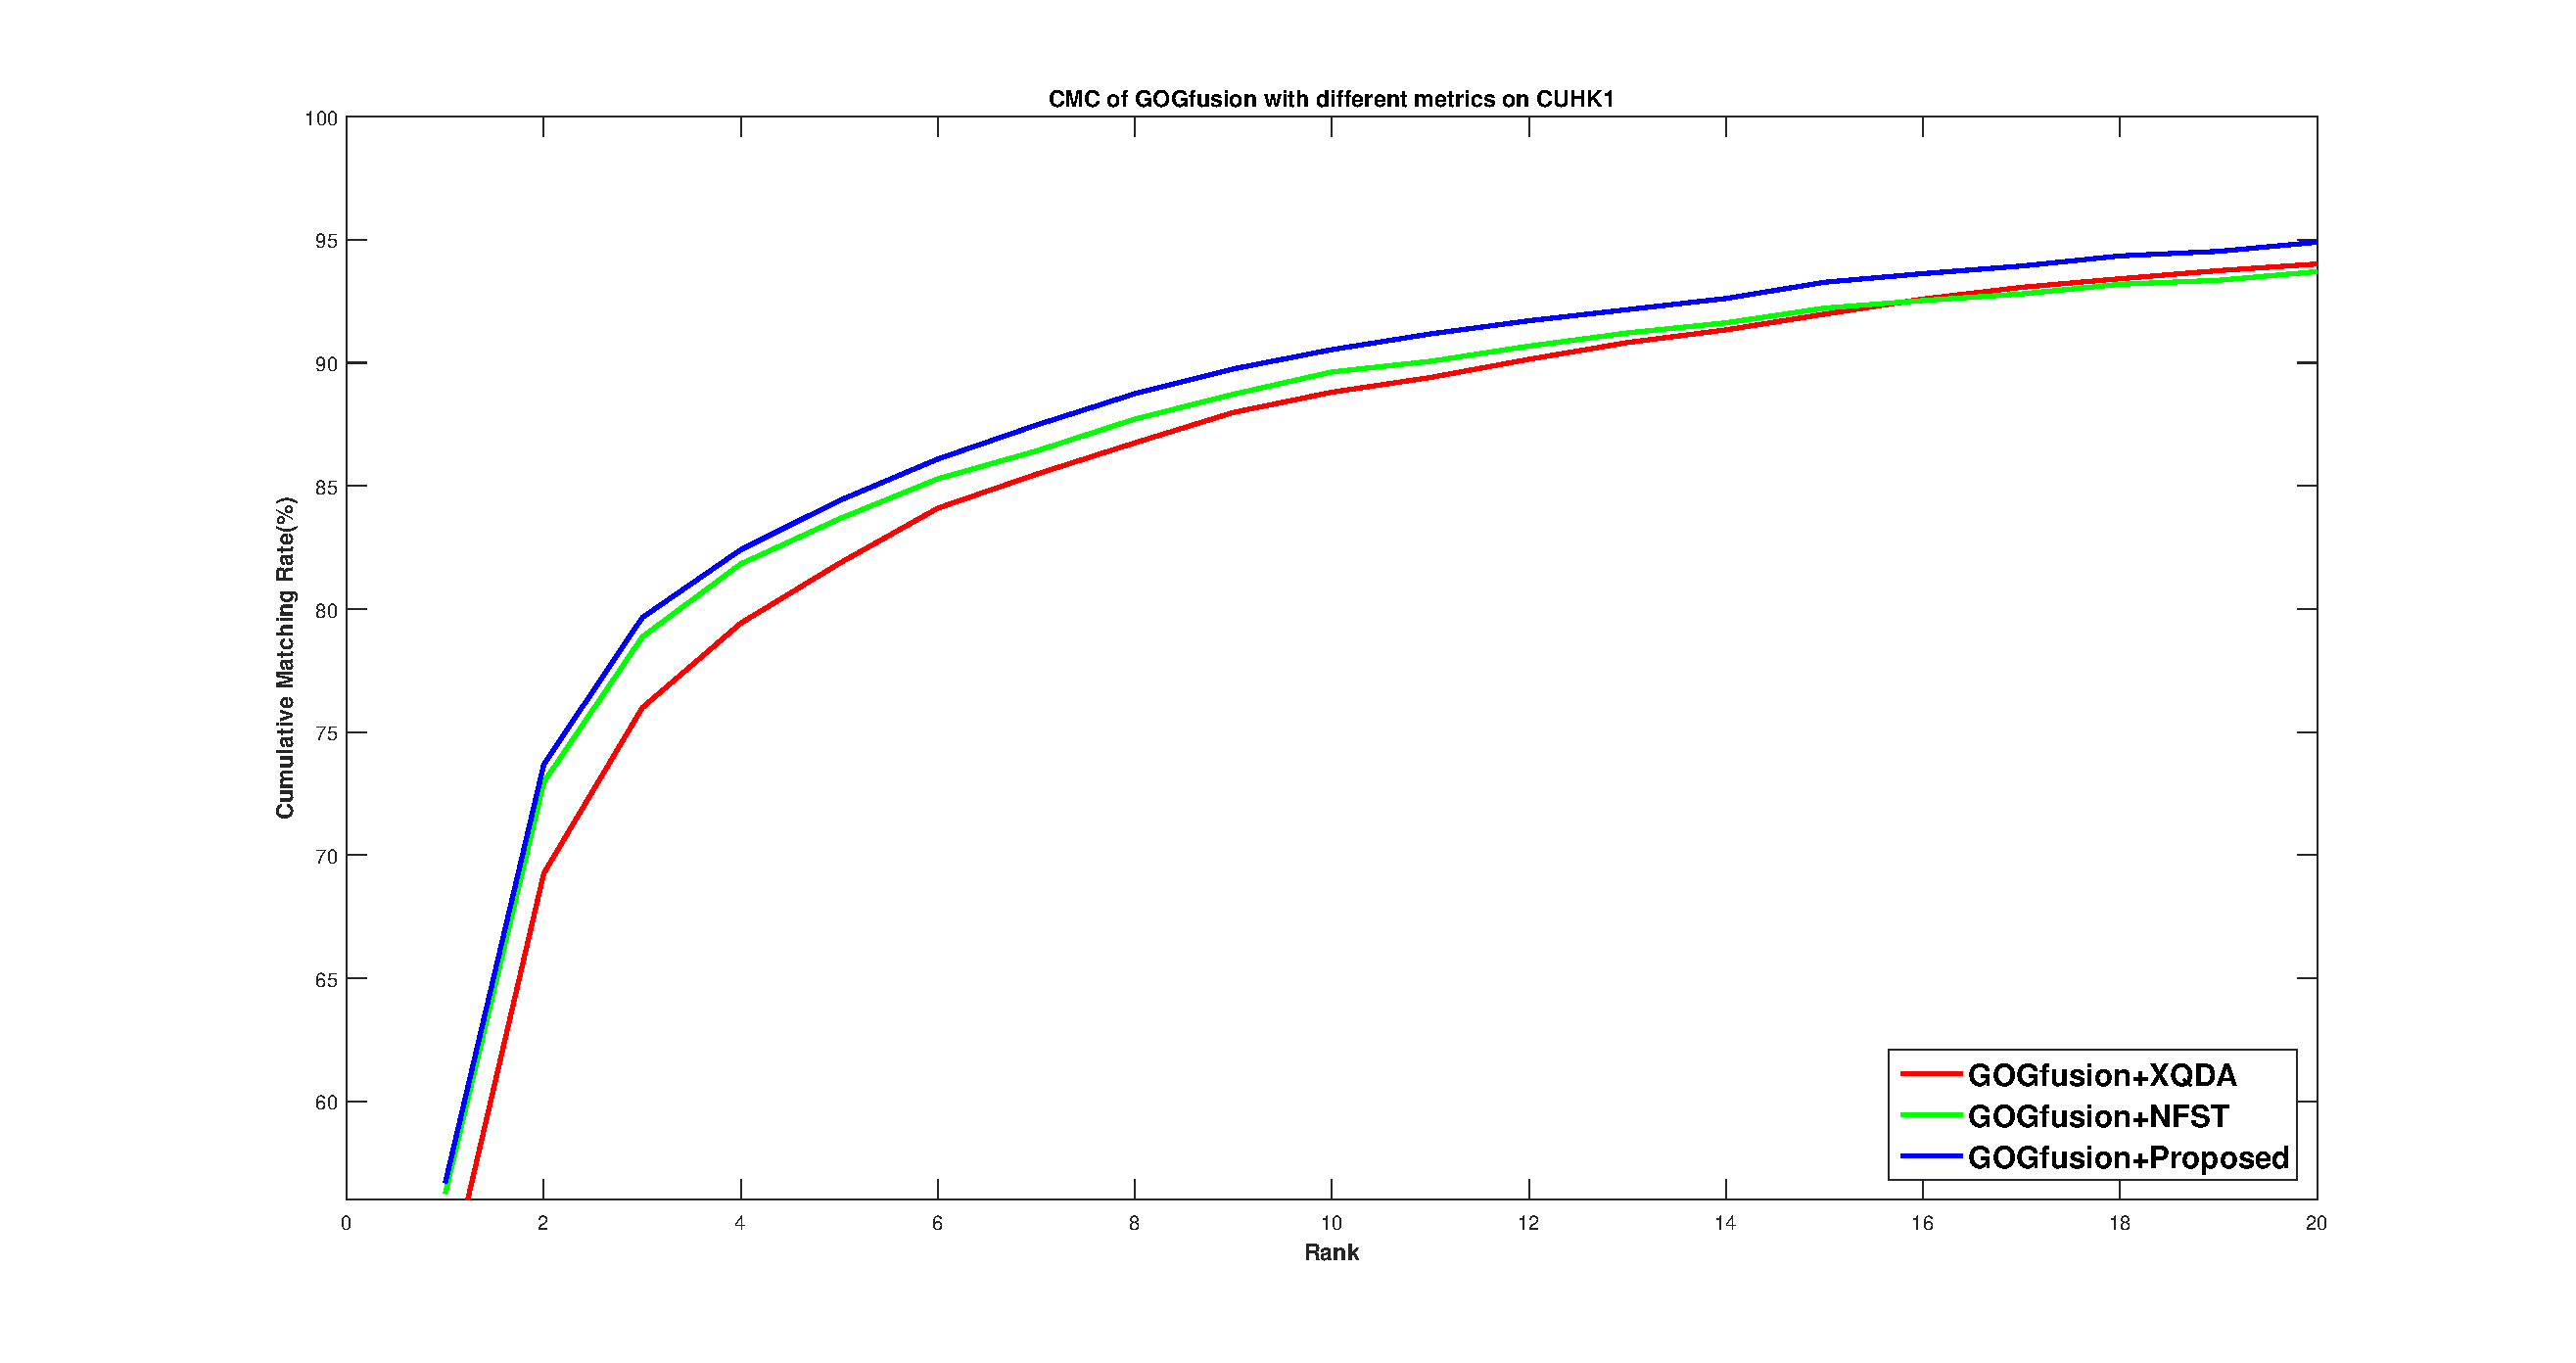
\includegraphics[width=1\linewidth]{/Users/JohnsonJohnson/Downloads/thesis_1/Figures/CUHK1.eps}
\vspace{-3em}
\caption{CMCs on CUHK1 comparing different metric learning}
%\end{raggedleft}
\end{figure}

%-----------------------------------------------------------------------PRID_2011


\begin{table}[H]
\centering
\caption{Performance of different metrics on prid\_2011}
\begin{tabular}{|l|c|c|c|c|c|c|}
\hline
& \multicolumn{5}{|c|}{Rank(\%)} \\
\hline
Methods& 1 & 5 &10& 15&20\\
\hline
GOG$_\text{rgb}$+NFST&26.60 &53.80& 62.90&71.30&75.40 \\ 
\hline
GOG$_\text{rgb}$+XQDA&31.10 & 55.70& 66.10 & 72.40&76.10\\  
\hline
%GOG$_\text{rgb}$+KLFDA&23.70&51.70&63.10&69.90&73.60\\ 
%\hline
GOG$_\text{rgb}$+Proposed&23.80&52.20&63.50&70.20&73.50\\  %23.80%, 52.10%, 63.50%, 70.20%, 73.50%
\hline
GOG$_\text{fusion}$+NFST&34.10 &58.30& 67.60&73.80&78.30 \\  
\hline
GOG$_\text{fusion}$+XQDA&38.40& 61.30&70.80&75.60&79.30\\
\hline
%GOG$_\text{fusion}$+KLFDA & 31.90&56.90&66.60&72.60&77.50\\
%\hline
GOG$_\text{fusion}$+Proposed&32.30&57.40&66.30&73.40&78.00\\ %32.20%, 57.50%, 66.40%, 73.50%, 78.00(alpha = 0.7)   ()% 32.20%, 57.50%, 66.40%, 73.50%, 78.00%(alpha = 0.8)

\hline

\end{tabular}\newline
\end{table}

\textbf{Prid\_2011}  The  rank 1, rank 5, rank 10, rank 15 and rank 20 scores of GOG$_\text{fusion}$  combined with proposed metric are 6.1\%, 3.9\%, 4.5\%, 2.2\% and 1.3\% lower than GOG$_\text{fusion}$ combined with XQDA. The performance of NFST is slightly better than proposed metric. Also, in terms of GOG$_\text{rgb}$, XQDA and NFST have better performance than the proposed one. So in this dataset, the proposed metric has worse performance than XQDA and NFST.

\begin{figure}[H]
\begin{raggedleft}
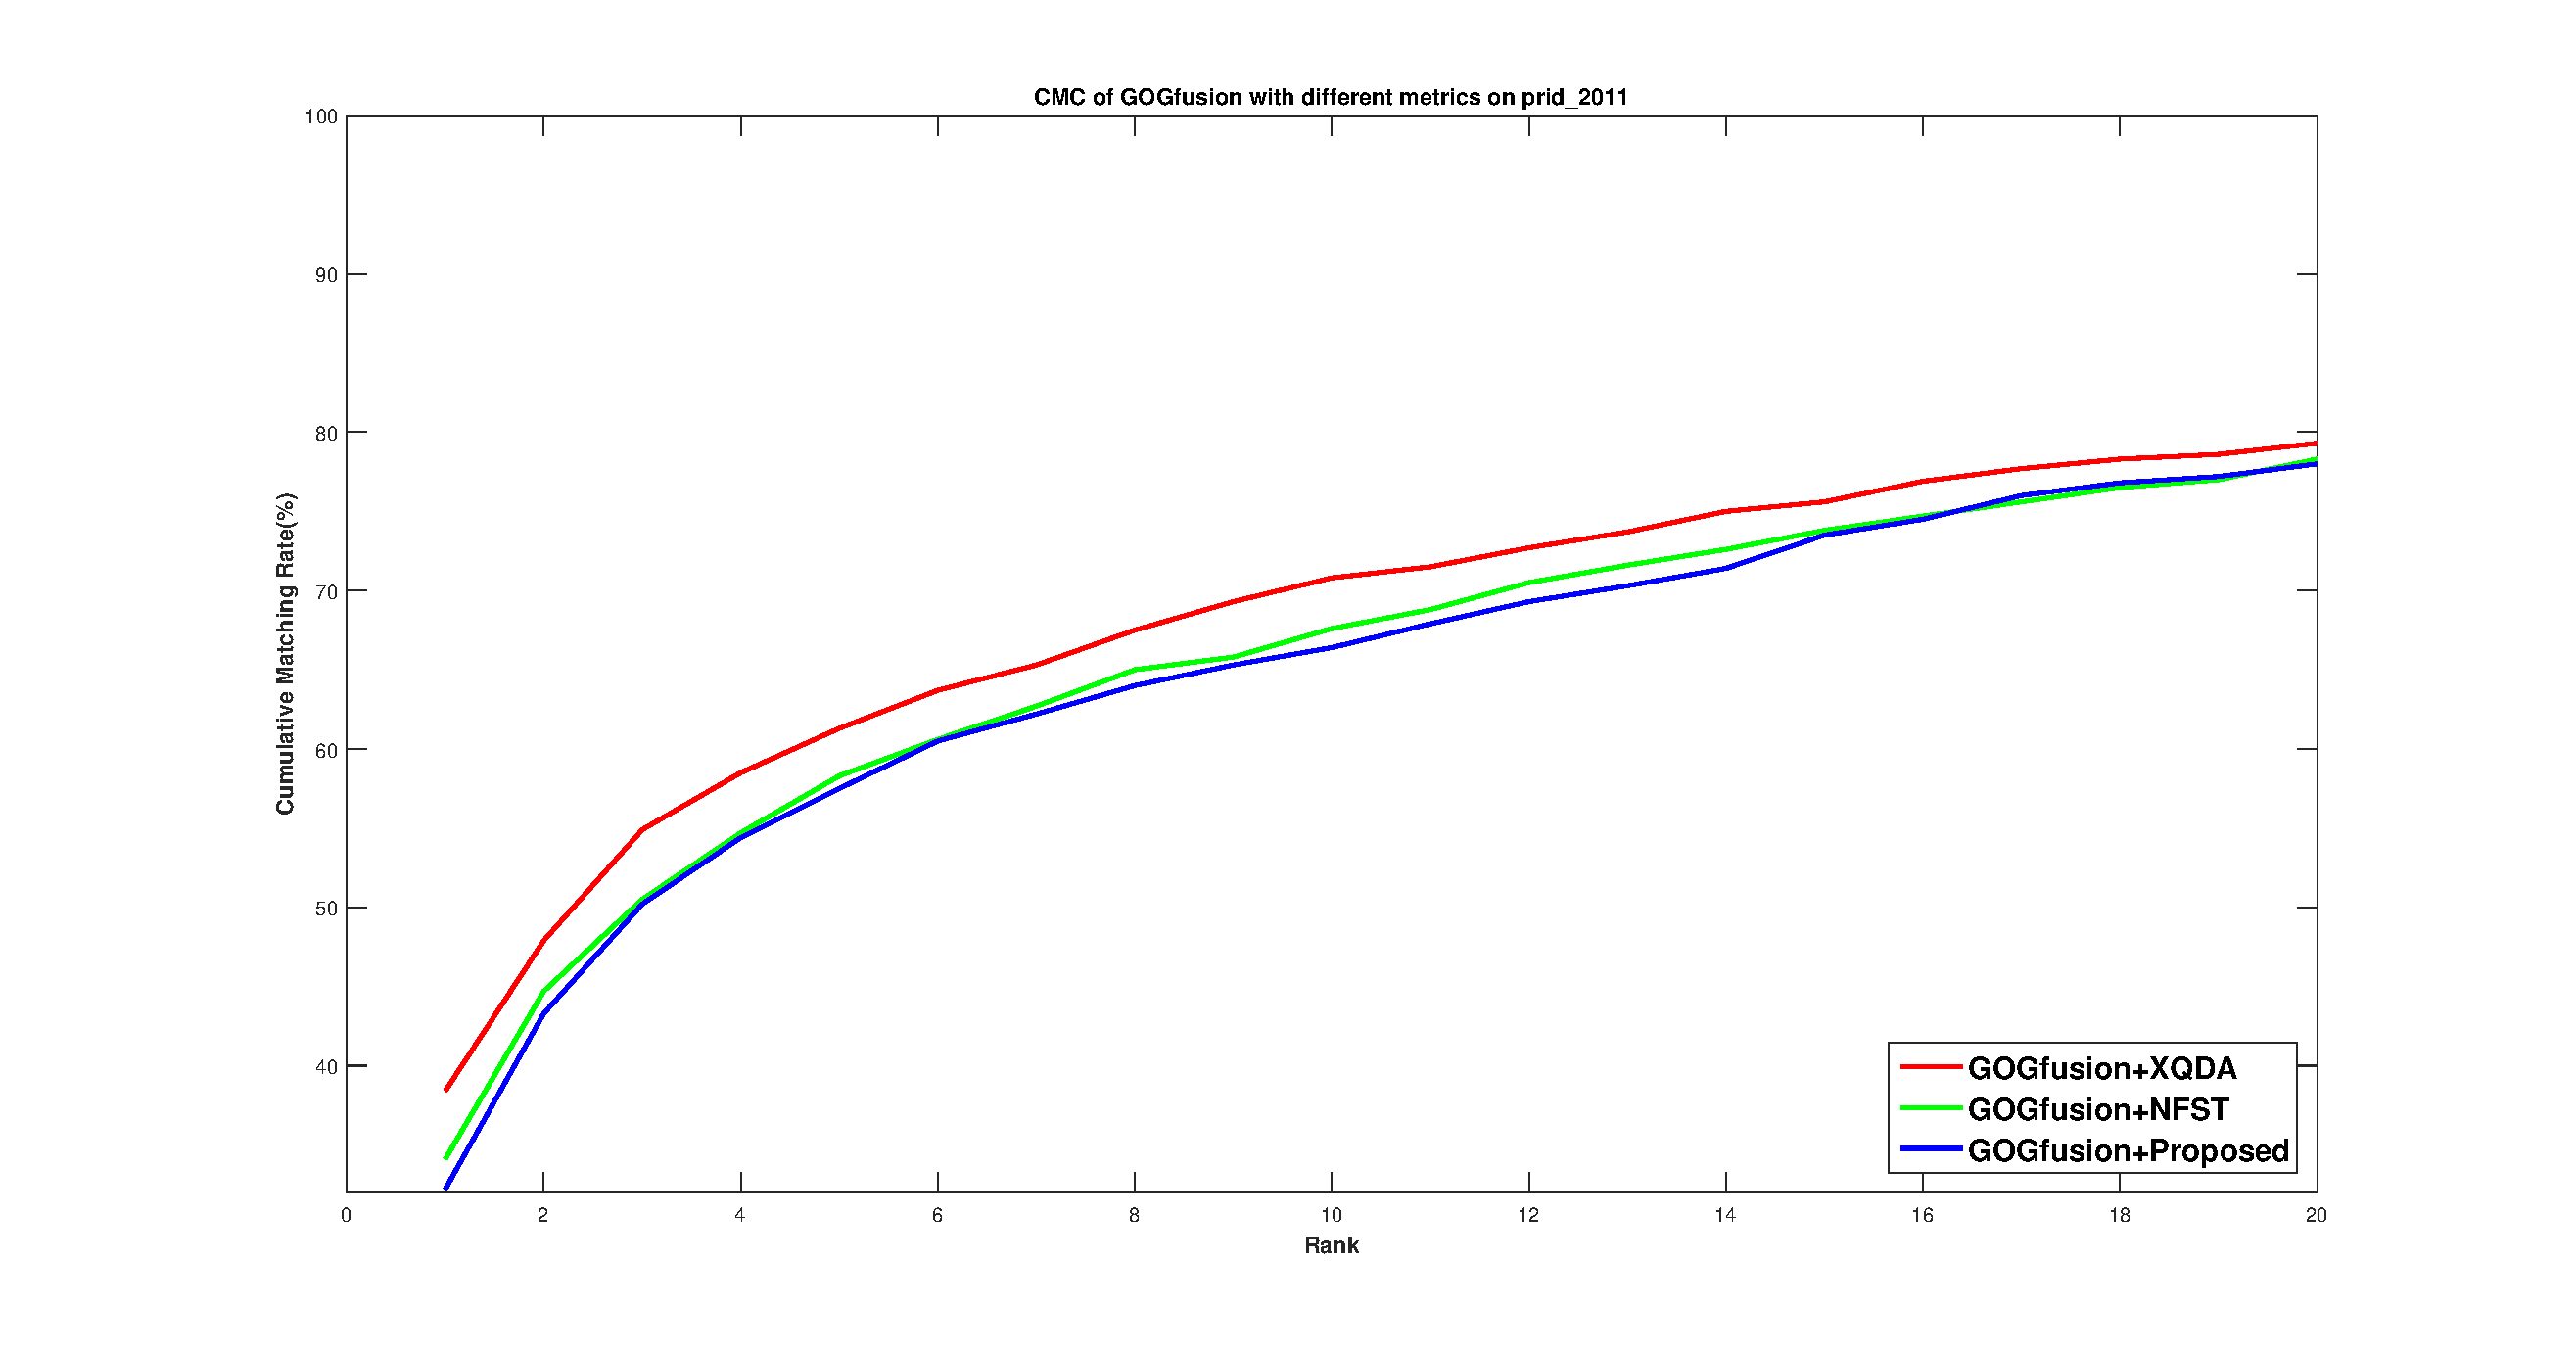
\includegraphics[width=1\linewidth]{/Users/JohnsonJohnson/Downloads/thesis_1/Figures/prid2011.eps}
\vspace{-3em}
\caption{CMCs on prid\_2011 comparing different metric learning}
\end{raggedleft}
\end{figure}

%-----------------------------------------------------------------------PRID_450S
\begin{table}[H]
\caption{Performance of different metrics on prid\_450s}
\centering
\begin{tabular}{|l|c|c|c|c|c|c|}
\hline
& \multicolumn{5}{|c|}{Rank(\%)} \\
\hline
Methods& 1 & 5 &10& 15&20\\
\hline
GOG$_\text{rgb}$+NFST& 61.96&84.98 &90.53& 94.09&96.09 \\  %61.96%, 84.98%, 90.53%, 94.09%, 96.09%
\hline
GOG$_\text{rgb}$+XQDA&65.29 &85.02 & 91.13&94.76& 96.49\\ 
\hline
%GOG$_\text{rgb}$+KLFDA&60.04&84.09&90.93&94.04&96.00 \\ 
%\hline
GOG$_\text{rgb}$+Proposed&60.71&84.53&91.29&94.13&96.27\\  %60.44%, 84.44%, 91.33%, 94.00%, 96.13%
\hline
GOG$_\text{fusion}$+NFST& 64.53&86.62 & 92.93&95.78&97.42 \\ 
\hline
GOG$_\text{fusion}$+XQDA&68.40 & 87.42&93.47 &95.69& 97.02\\ 
\hline
%GOG$_\text{fusion}$+KLFDA & 62.58&86.18&92.18&95.11&96.84\\
%\hline
GOG$_\text{fusion}$+Proposed&62.80&86.58&92.36&95.29& 96.89\\ % 62.62%, 86.44%, 92.36%, 95.20%, 96.93%(alpha = 0.7) 62.89%, 86.49%, 92.49%, 95.29%, 97.07%(alpha = 0.8)

\hline

\end{tabular}
\end{table}
\textbf{Prid\_450s} In this dataset, we can find that the rank 1 score of XQDA and NFST is higher than the proposed metric, but those three metrics have almost the same rank 5, rank 10, rank 15, and rank 20 scores with respect to both kinds of descriptors.  

\begin{figure}[H]
\begin{raggedleft}
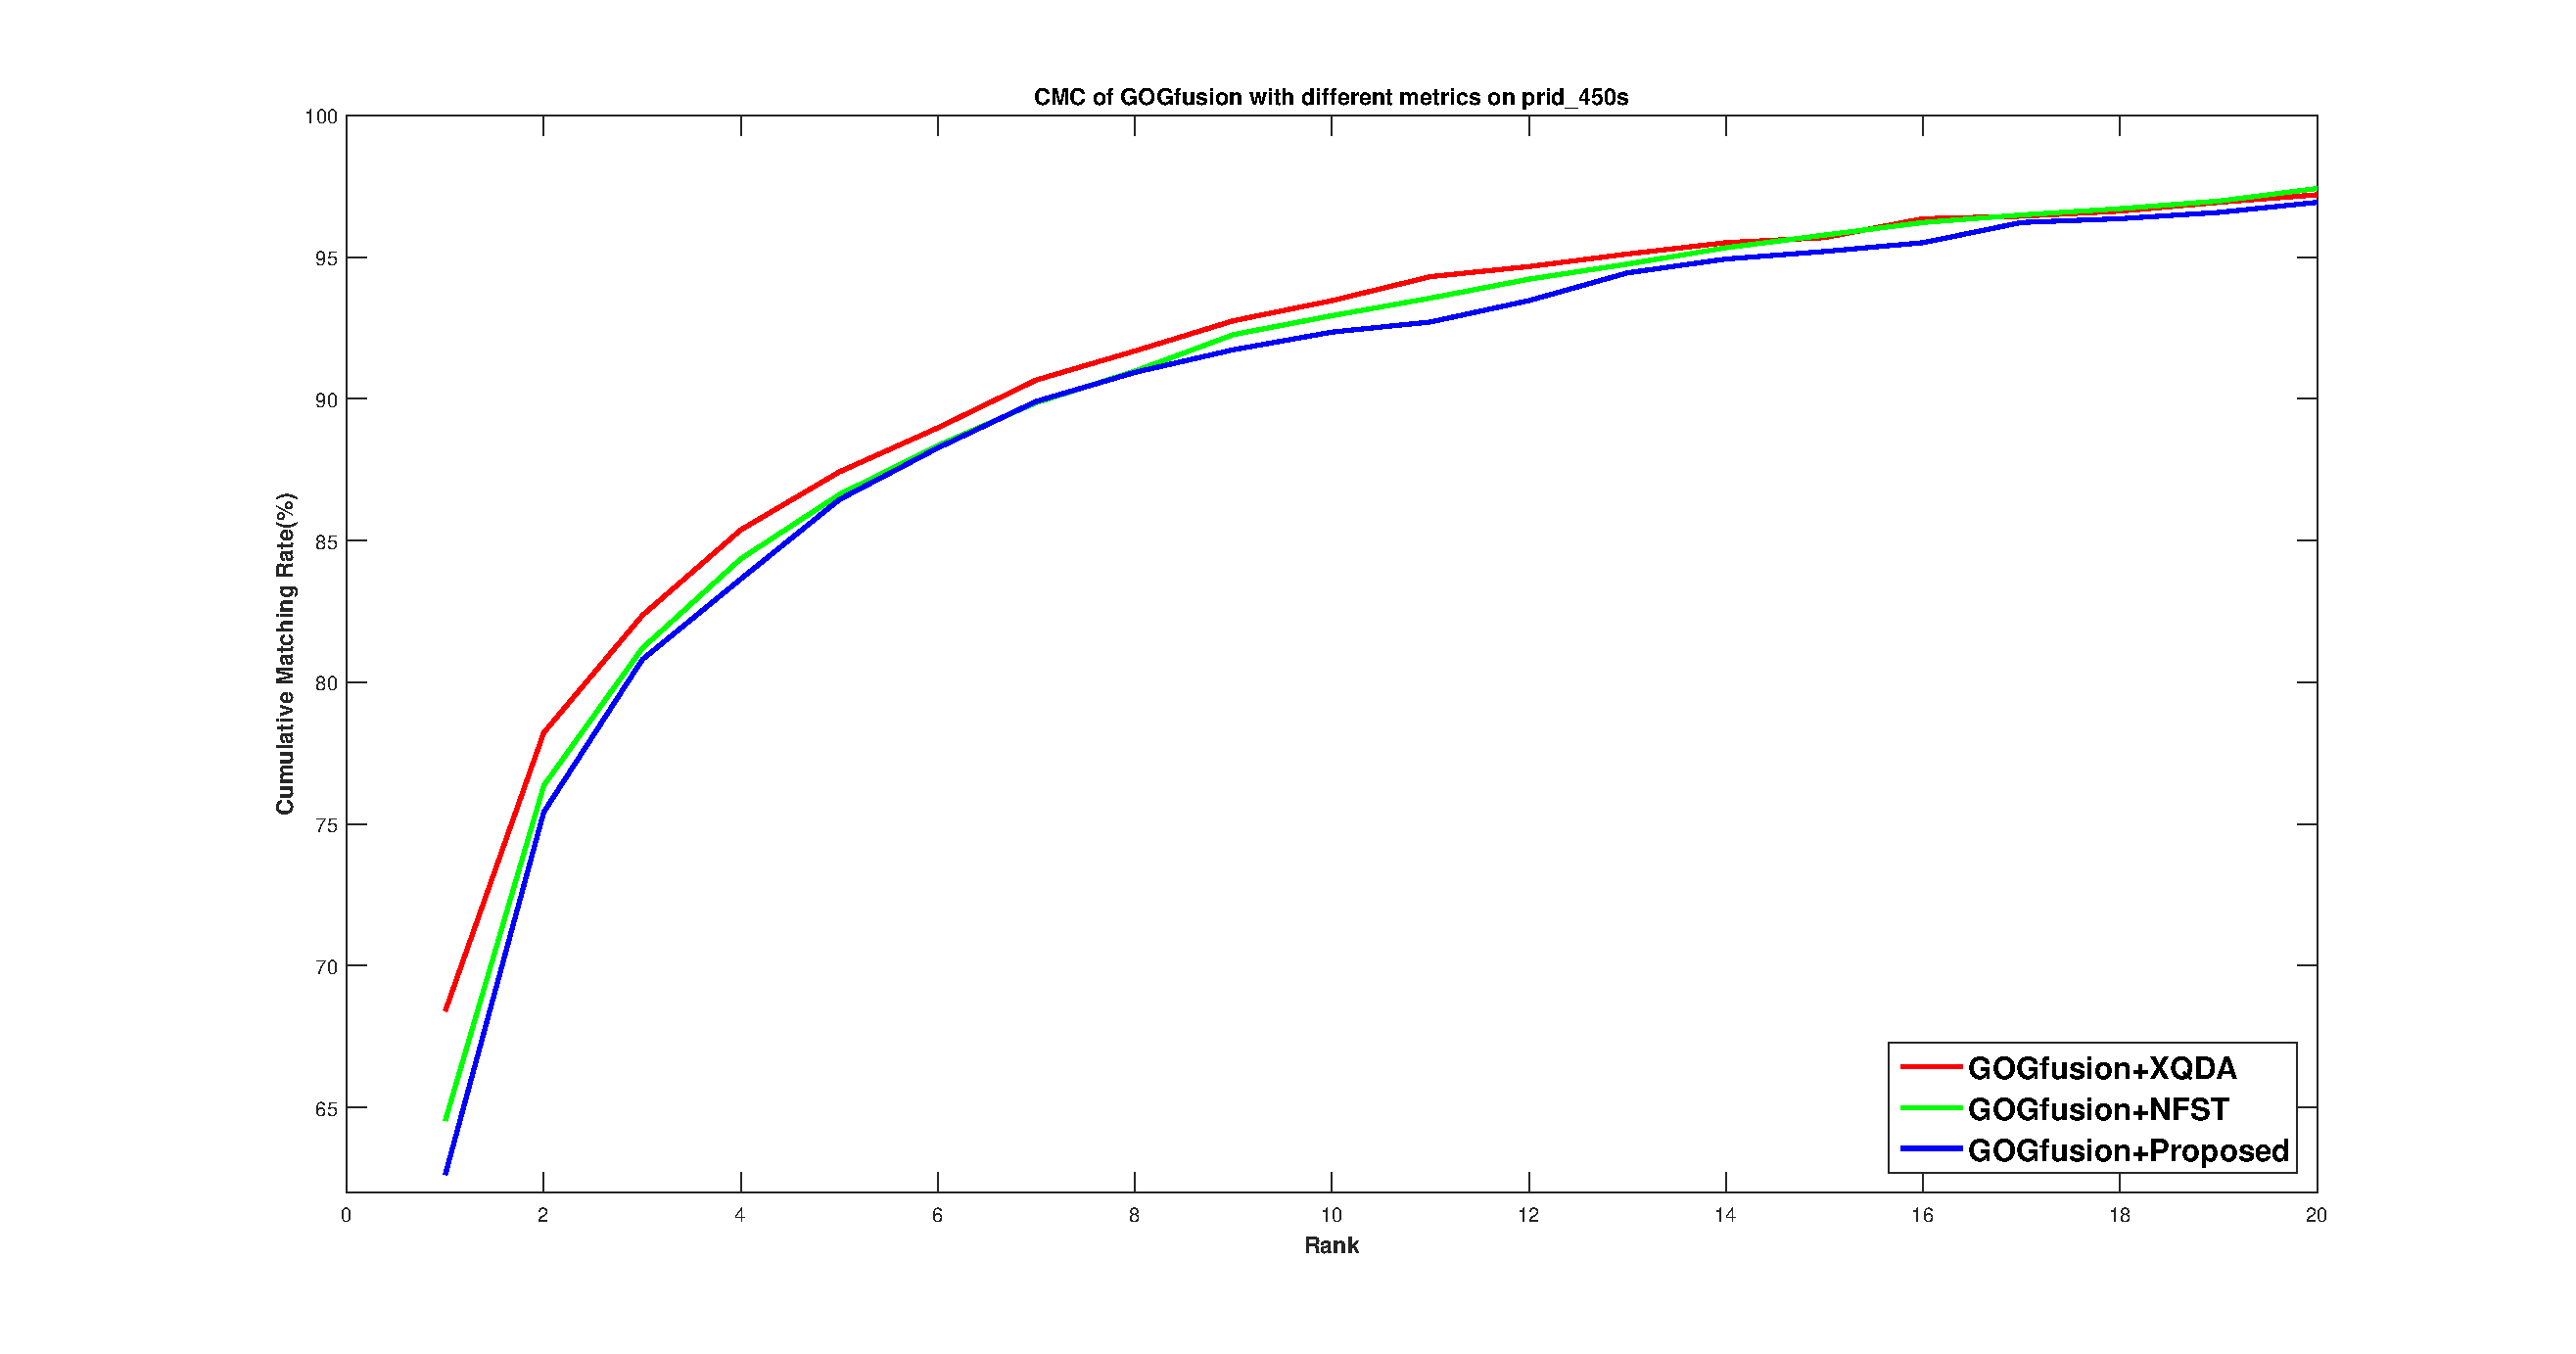
\includegraphics[width=1\linewidth]{/Users/JohnsonJohnson/Downloads/thesis_1/Figures/prid450s.eps}
\vspace{-3em}
\caption{CMCs on prid\_450s comparing different metric learning}
\end{raggedleft}
\end{figure}

%-----------------------------------------------------------------------GRID
\begin{table}[H]
\caption{Performance of different metrics on GRID}
\centering
\begin{tabular}{|l|c|c|c|c|c|c|}
\hline
& \multicolumn{5}{|c|}{Rank(\%)} \\
\hline
Methods& 1 & 5 &10& 15&20\\
\hline
GOG$_\text{rgb}$+NFST& 21.84&41.28 &50.96& 57.44&62.88 \\ 
\hline
GOG$_\text{rgb}$+XQDA& 22.64&43.92 &55.12 &61.12&66.56\\ 
\hline
%GOG$_\text{rgb}$+KLFDA&23.44&43.04&52.16&59.12&64.88 \\ 
%\hline
GOG$_\text{rgb}$+Proposed&22.64&43.68&52.00&59.04&65.04\\  %22.80%, 43.76%, 52.08%, 59.04%, 65.12%
\hline
GOG$_\text{fusion}$+NFST& 23.04&44.40 &54.40 &61.84&66.56\\ 
\hline
GOG$_\text{fusion}$+XQDA& 23.68&47.28 &58.40 &65.84&69.68 \\ 
\hline
%GOG$_\text{fusion}$+KLFDA &23.76&44.40& 55.36&61.76& 66.48\\
%\hline
GOG$_\text{fusion}$+Proposed&23.92&44.64&54.88&62.32&66.40\\ %23.84%, 44.64%, 55.04%, 62.24%, 66.24%

\hline

\end{tabular}
\end{table}

\begin{figure}[H]
\begin{raggedleft}
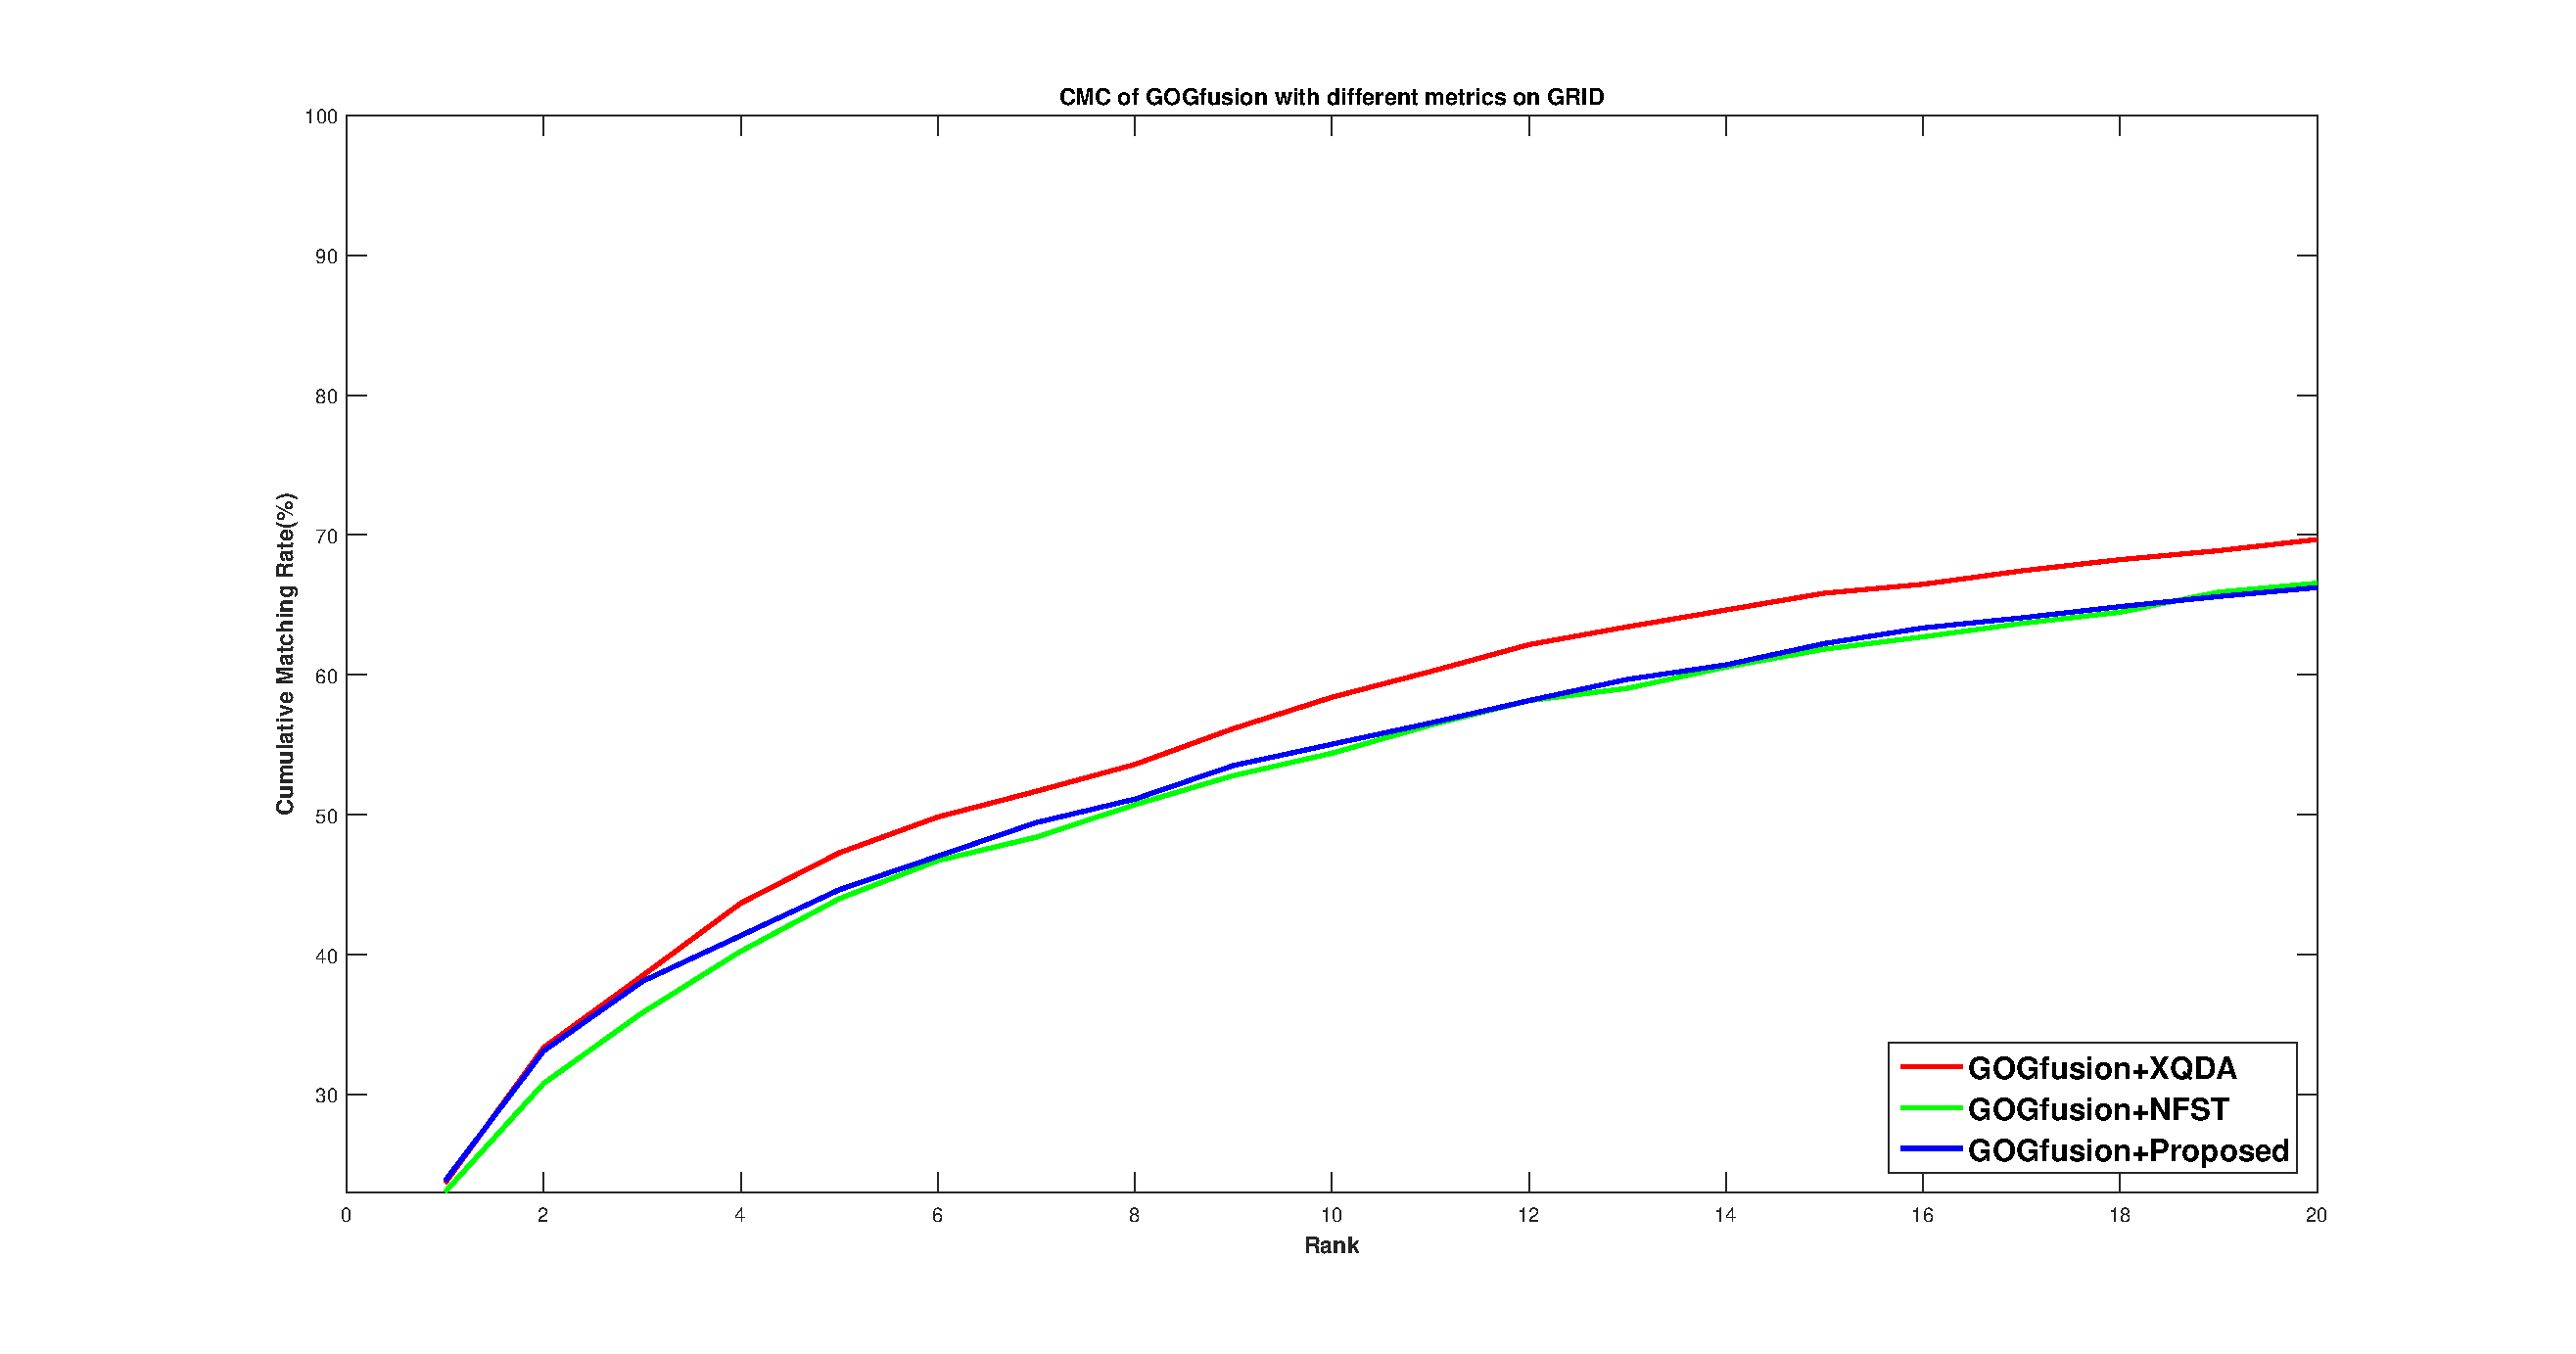
\includegraphics[width=1\linewidth]{/Users/JohnsonJohnson/Downloads/thesis_1/Figures/GRID.eps}
\vspace{-3em}
\caption{CMCs on GRID comparing different metric learning}
\end{raggedleft}
\end{figure}

\textbf{GRID} We can see that the rank 1 score of proposed metric is 0.24\% higher than XQDA and 0.88\% higher than NFST in terms of GOG$_\text{fusion}$, but XQDA outperforms proposed metric on rank 5, rank 10, rank 15 and rank 20 scores. Besides, proposed metric outperforms NFST on rank 5, rank 10 and rank 15 scores.\\
\indent In summary, our proposed metric improved the Re-ID accuracy in VIPeR and CUHK1 datasets, and has almost the same performance with NFST and XQDA in the prid\_450s dataset. Specifically, the proposed metric learning has the best rank 1 score in the GRID dataset and its performance is only second to XQDA. The proposed metric has superior performance for the following reasons: (1) dimension reduction by KLFDA exploits the nonlinearity, and the loss of discriminant information between classes is minimized; (2) the simplified relative distance limitation optimization helps to confine the Mahalanobis distance matrix $\bm{M}$ to discriminate different classes.  
%------------------------------------------------------------------------

